\section{Background Estimation}
\label{sec:backgroundestimation}

\subsection{Data-Driven Background Estimation Using the \texorpdfstring{\twoxtwod}{2x2D} Sidebands}


\subsubsection{Description of the \twoxtwod\ Sideband Method}
\label{subsec:2x2ddescriptionmethod}

The double-two-dimensional (\twoxtwod) sidebands method \cite{STDM-2011-05} is a standard method for estimating the composition of the background in diphoton events. The same procedure is employed as in the two previous measurements at 13 \TeV \cite{HIGG-2019-13} and 13.6 \TeV (31.4 \ifb) \cite{HIGG-2022-12}. The procedure is described in detail in the Internal Notes \cite{HIGG-2019-13-INT1,HIGG-2022-10-INT1}.

The main sources of background are the non-resonant production of prompt and isolated diphotons ($\gamma \gamma$) and the $\gamma j$ and $jj$ processes where one or two hadronic jets are misidentified as photons. 

In the \twoxtwod\ method, the identification and isolation requirements for the photons are loosened. Only events passing the \texttt{LoosePrime3} working point are considered in the nominal result. This criterion is defined by relaxing three strip variables ($\omega_{s3}$, $F_\mathrm{side}$ and $\Delta E$) with respect to the Tight criterion. Details of the photon identification variables are given in \cite{PERF-2017-02}.

The events are separated into 16 orthogonal regions, defined by whether one or both photons pass or fail the nominal identification and isolation requirements. The \(\gamma\gamma\), \(\gamma j\) and \(jj\) yields after the nominal selection are obtained by solving a system of equations, given the observed yields in the 16 regions, as well as the photon identification and isolation efficiencies as estimated from MC simulation. 

The fractions contributed by the \(\gamma\gamma\), \(\gamma j\) and \(jj\) background sources after the inclusive diphoton selection are \SI{66.9}{\percent}, \SI{28.8}{\percent} and \SI{4.4}{\percent}, respectively, as shown in Table \ref{tab:2x2dsidebands202224}. 

%%% Only showing stat uncertainties for now
% Systematic uncertainty on the background fractions is estimated by varying the loosened identification pre-selection from \texttt{LoosePrime3} to \texttt{LoosePrime4} and \texttt{LoosePrime5}. Both aalternative WPs require an additional cut on the variable $E_\mathrm{ratio}$ and, in addition, \texttt{LoosePrime5} imposes a cut on $w_\mathrm{s\,tot}$. 
\ASnote{Include figure/tables with systematics evaluated}

% The systematic uncertainties in the measured background fractions are due to the definition of the control regions arising from the different inverted photon identification criteria, as shown in [TODO: Systematics]. 
% But these systematic uncertainties are not propagated further to the analysis. 
% ALEX: What shall we do with systematic uncertainties? Discuss with Liza and Luis.


\subsubsection{Plots and Tables}
\label{subsec:2x2dtables}

Tables showing the inclusive background fractions for the 2022, 2023, and 2024 data are shown in \ref{tab:2x2dsidebands2022}, \ref{tab:2x2dsidebands2023}, and \ref{tab:2x2dsidebands2024}.

\newpage
\FloatBarrier

\begin{table}[!h]
    \centering
    \caption{Background decomposition using the \twoxtwod\ sidebands method for 2022-2024 data and \texttt{mc23a-e}.}
    \includegraphics[width=\textwidth,page=2,trim={4.6cm 24.9cm 4.6cm 3.5cm},clip]{figures/2x2d_sidebands/sb_out_2022-24/table_HGam2x2DBkgDecomp_Xsection_SpringPaper.pdf}
    \label{tab:2x2dsidebands202224}
\end{table}


\begin{table}[!h]
    \centering
    \caption{Background decomposition using the \twoxtwod\ sidebands method for 2022 data and \texttt{mc23a}.}
    \includegraphics[width=\textwidth,page=2,trim={4.85cm 24.9cm 4.85cm 3.5cm},clip]{figures/2x2d_sidebands/sb_h032_2022_debug/table_HGam2x2DBkgDecomp_Xsection_SpringPaper.pdf}
    \label{tab:2x2dsidebands2022}
\end{table}


\begin{table}[!h]
    \centering
    \caption{Background decomposition using the \twoxtwod\ sidebands method for 2023 data and \texttt{mc23d}.}
    \includegraphics[width=\textwidth,page=2,trim={4.85cm 24.9cm 4.85cm 3.5cm},clip]{figures/2x2d_sidebands/sb_h032_2023_debug/table_HGam2x2DBkgDecomp_Xsection_SpringPaper.pdf}
    \label{tab:2x2dsidebands2023}
\end{table}


\begin{table}[!h]
    \centering
    \caption{Background decomposition using the \twoxtwod\ sidebands method for 2024 data and \texttt{mc23e}.}
    \includegraphics[width=\textwidth,page=2,trim={4.6cm 24.9cm 4.6cm 3.5cm},clip]{figures/2x2d_sidebands/sb_h032_2024_debug/table_HGam2x2DBkgDecomp_Xsection_SpringPaper.pdf}
    \label{tab:2x2dsidebands2024}
\end{table}


\begin{figure}[!h]
    \centering
    \includegraphics[width=\textwidth]{figures/2x2d_sidebands/sb_out_2022-24/plots/plot_bkgDecomp_Inclusive_inclusive.pdf}
    \label{fig:2x2dinclusive202224}
    \caption{Inclusive background yields for 2022--2024 data (\texttt{mc23a--e}).}
\end{figure}

% \begin{figure}[!h]
%     \centering
%     \begin{subfigure}{0.45\textwidth}
%         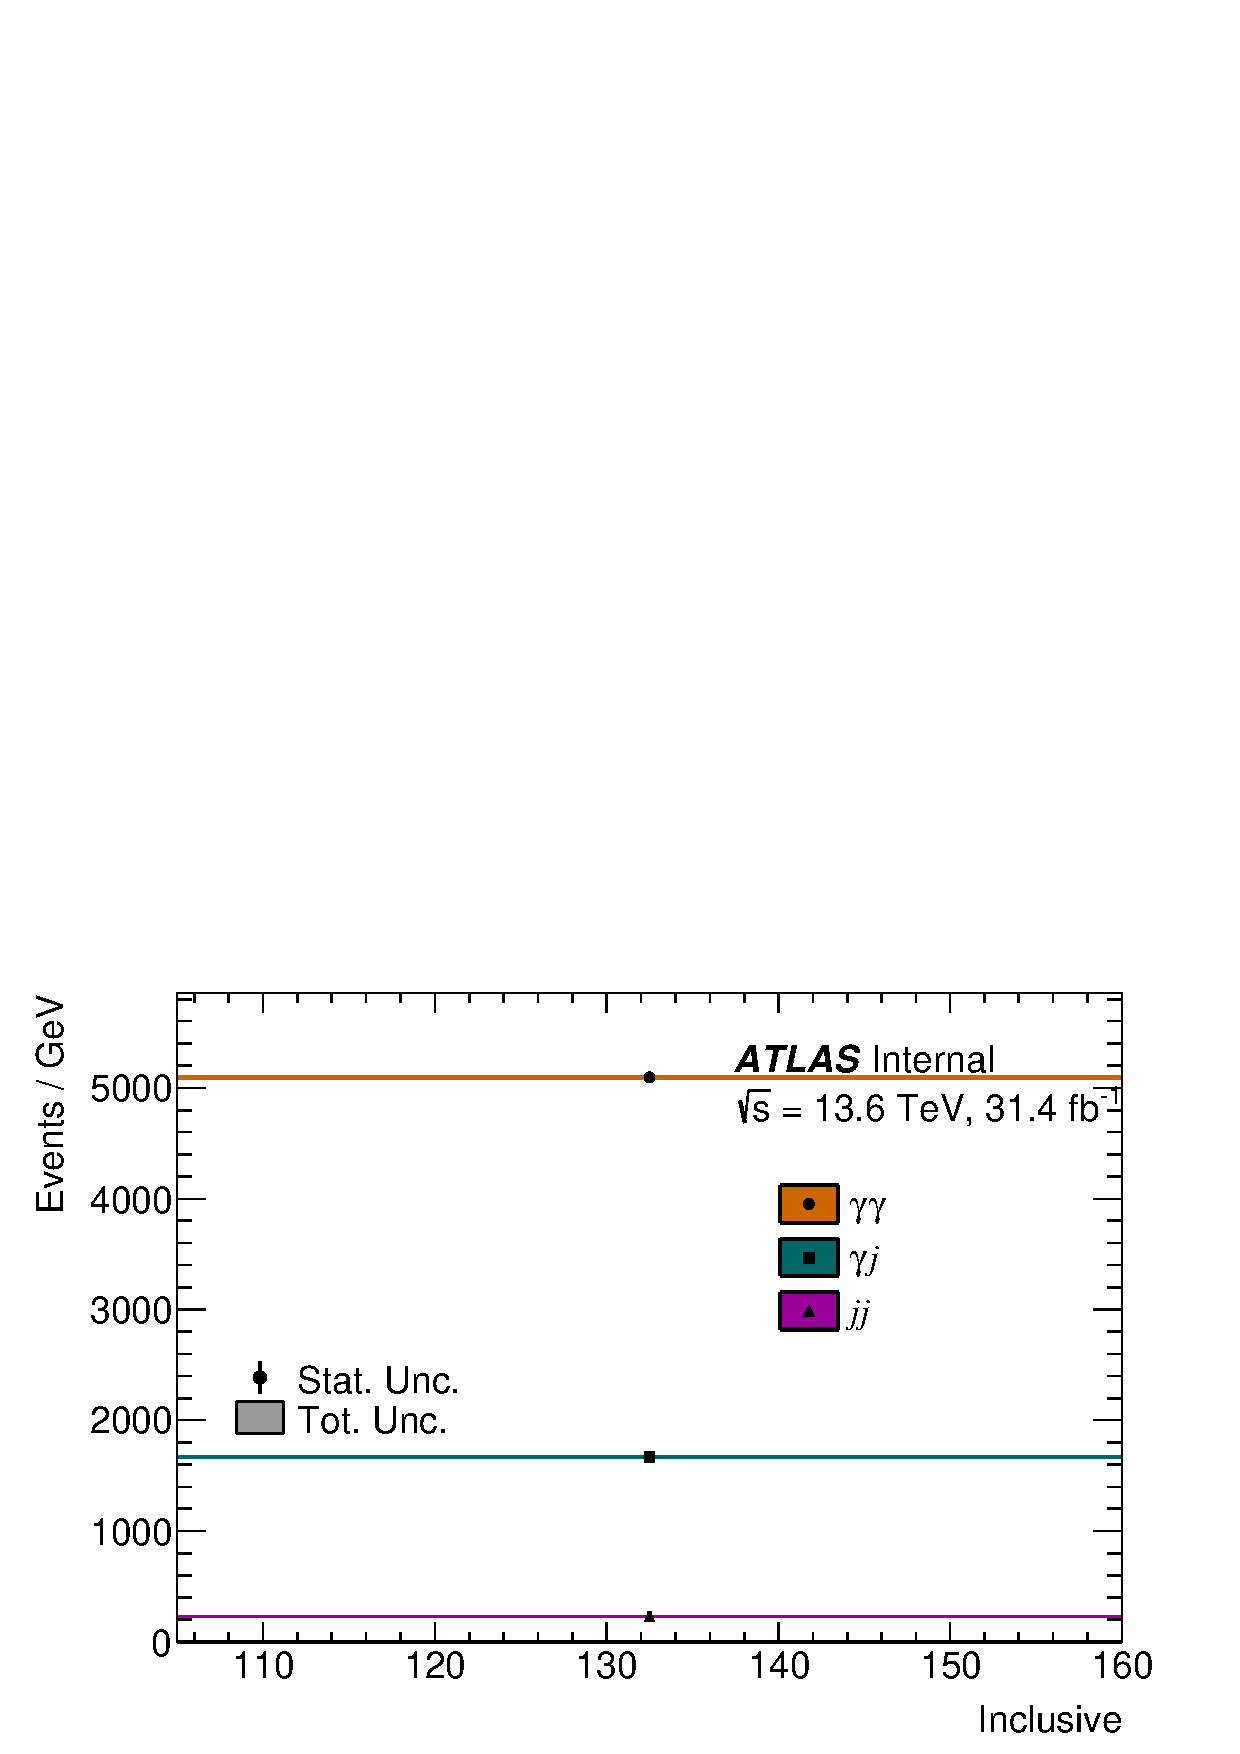
\includegraphics[width=\textwidth]{figures/2x2d_sidebands/sb_h032_2022_debug/plots/plot_bkgDecomp_Inclusive_inclusive.pdf}
%         \label{fig:2x2dinclusive2022}
%     \end{subfigure}
%     \begin{subfigure}{0.45\textwidth}
%         \includegraphics[width=\textwidth]{figures/2x2d_sidebands/sb_h032_2023_debug/plots/plot_bkgDecomp_Inclusive_inclusive.pdf}
%         \label{fig:2x2dinclusive2023}
%     \end{subfigure}
%     \begin{subfigure}{0.45\textwidth}
%         \includegraphics[width=\textwidth]{figures/2x2d_sidebands/sb_h032_2024_debug/plots/plot_bkgDecomp_Inclusive_inclusive.pdf}
%         \label{fig:2x2dinclusive2024}
%     \end{subfigure}
%     \begin{subfigure}{0.45\textwidth}
%         \includegraphics[width=\textwidth]{figures/2x2d_sidebands/sb_out_2022-24/plots/plot_bkgDecomp_Inclusive_inclusive.pdf}
%         \label{fig:2x2dinclusive2024}
%     \end{subfigure}
%     \caption{Inclusive background yields for 2022 (a), 2023 (b) and 2024 (c) data (\texttt{mc23a}, \texttt{mc23d} and \texttt{mc23e}).}
% \end{figure}


\begin{figure}[!h]
    \centering
    \includegraphics[width=\textwidth]{figures/2x2d_sidebands/sb_out_2022-24/plots/plot_purity_inclusive.pdf}
    \label{fig:2x2dpurinclusive202224}
    \caption{Inclusive background purity for 2022--2024 data (\texttt{mc23a--e}).}
\end{figure}

% \begin{figure}[!h]
%     \centering
%     \begin{subfigure}{0.45\textwidth}
%         \includegraphics[width=\textwidth]{figures/2x2d_sidebands/sb_h032_2022_debug/plots/plot_purity_inclusive.pdf}
%         \label{fig:2x2dpurinclusive2022}
%     \end{subfigure}
%     \begin{subfigure}{0.45\textwidth}
%         \includegraphics[width=\textwidth]{figures/2x2d_sidebands/sb_h032_2023_debug/plots/plot_purity_inclusive.pdf}
%         \label{fig:2x2dpurinclusive2023}
%     \end{subfigure}
%     \begin{subfigure}{0.45\textwidth}
%         \includegraphics[width=\textwidth]{figures/2x2d_sidebands/sb_h032_2024_debug/plots/plot_purity_inclusive.pdf}
%         \label{fig:2x2dpurinclusive2024}
%     \end{subfigure}
%     \caption{Inclusive background purity for 2022 (a), 2023 (b) and 2024 (c) data (\texttt{mc23a}, \texttt{mc23d} and \texttt{mc23e}).}
% \end{figure}


\begin{figure}[!h]
    \centering
    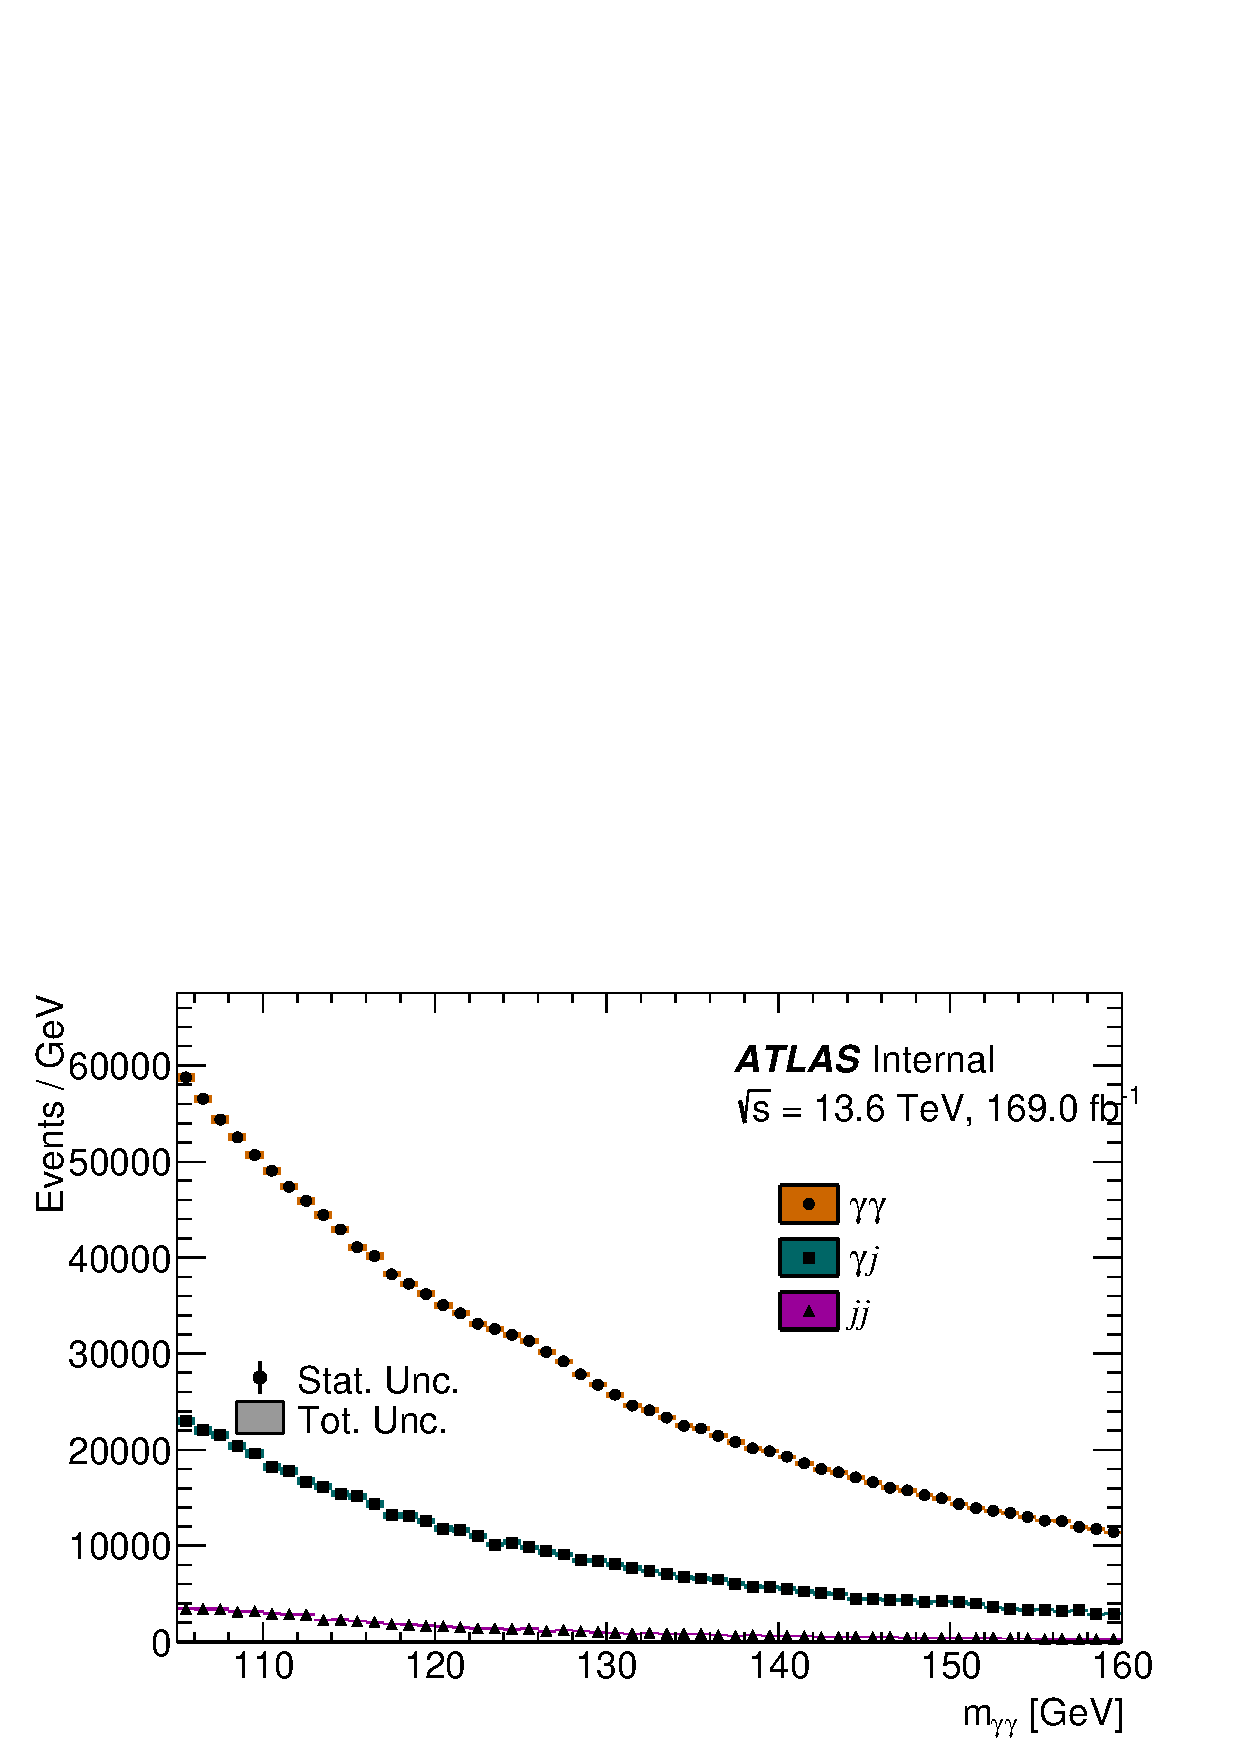
\includegraphics[width=\textwidth]{figures/2x2d_sidebands/sb_out_2022-24/plots/plot_bkgDecomp_Inclusive_m_yy.pdf}
    \label{fig:2x2dmyy202224}
    \caption{Background yields as a function of $m_{\gamma \gamma}$ for 2022--2024 data (\texttt{mc23a--e}).}
\end{figure}

% \begin{figure}[!h]
%     \centering
%     \begin{subfigure}{0.45\textwidth}
%         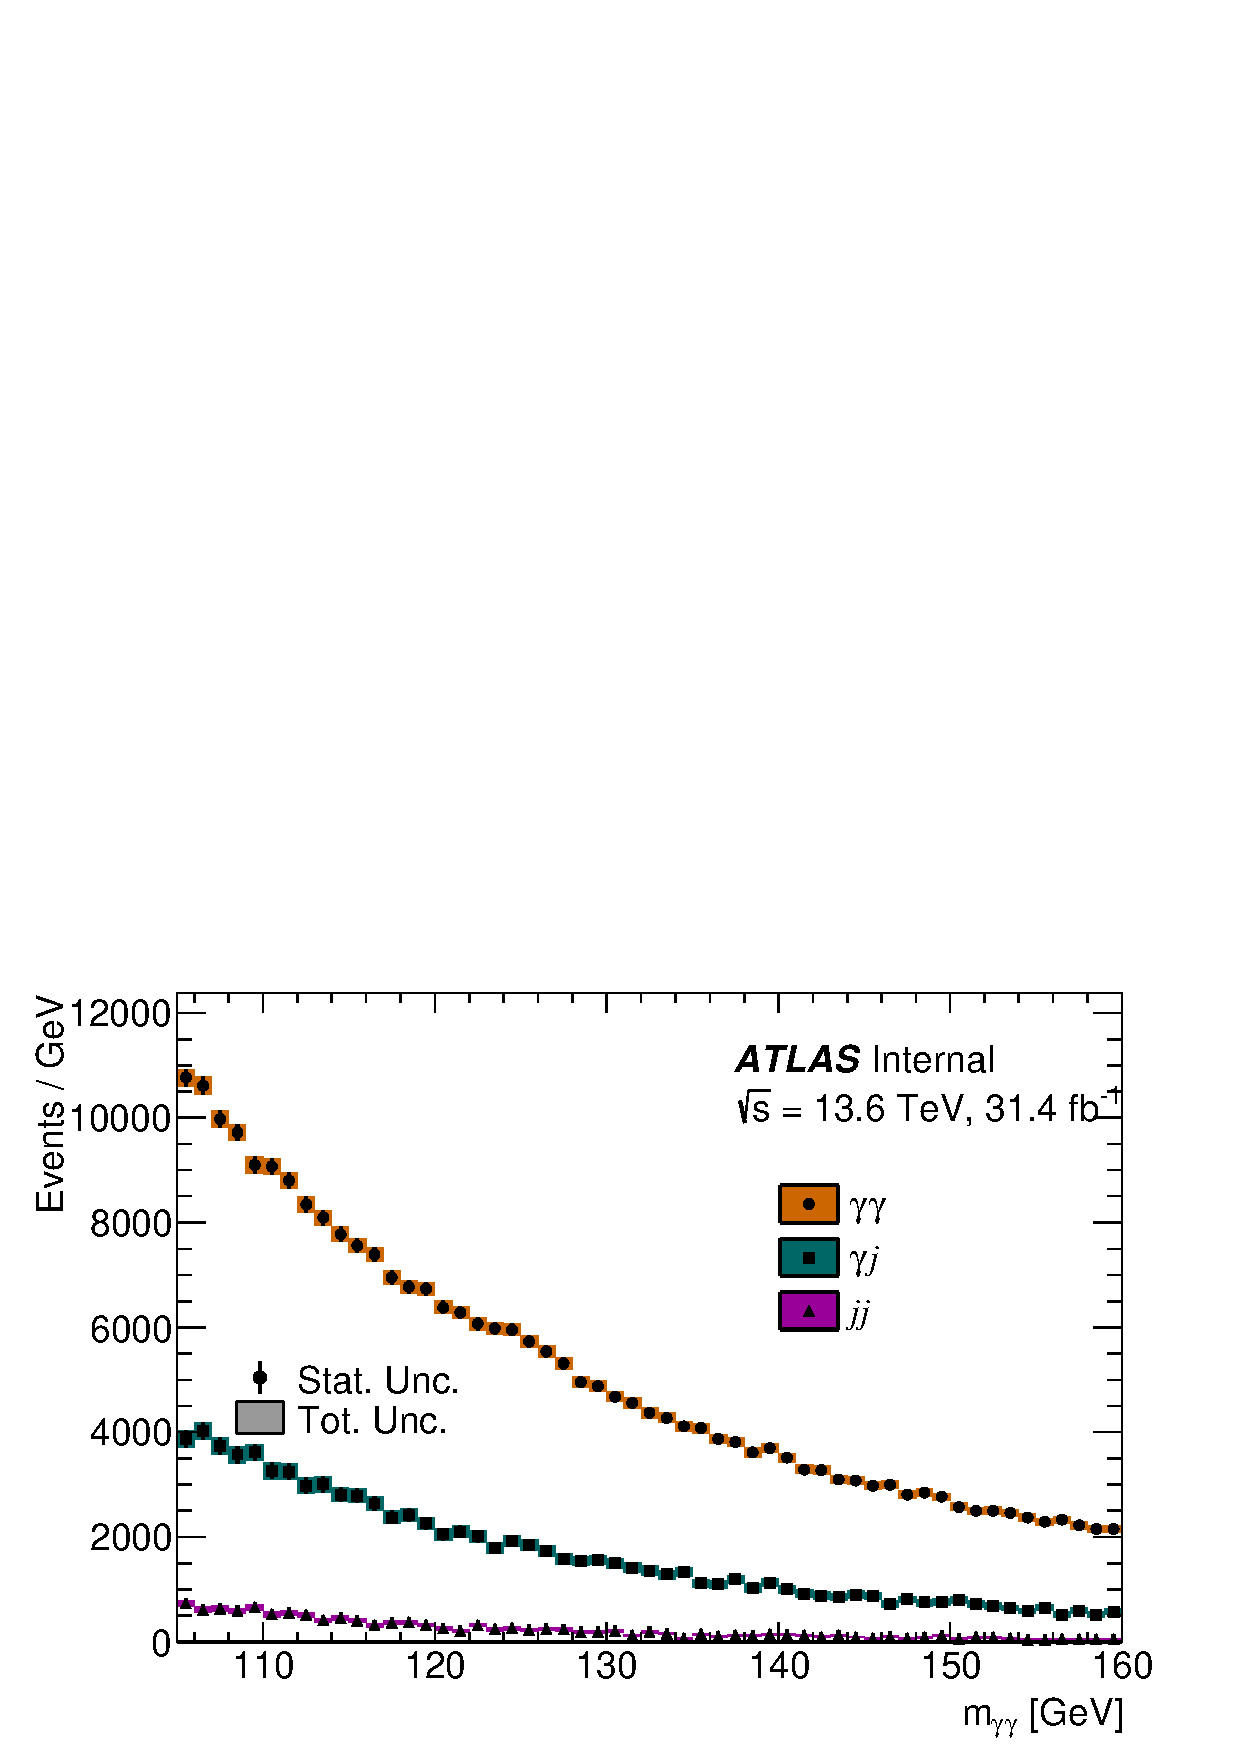
\includegraphics[width=\textwidth]{figures/2x2d_sidebands/sb_h032_2022_debug/plots/plot_bkgDecomp_Inclusive_m_yy.pdf}
%         \label{fig:2x2dmyy2022}
%     \end{subfigure}
%     \begin{subfigure}{0.45\textwidth}
%         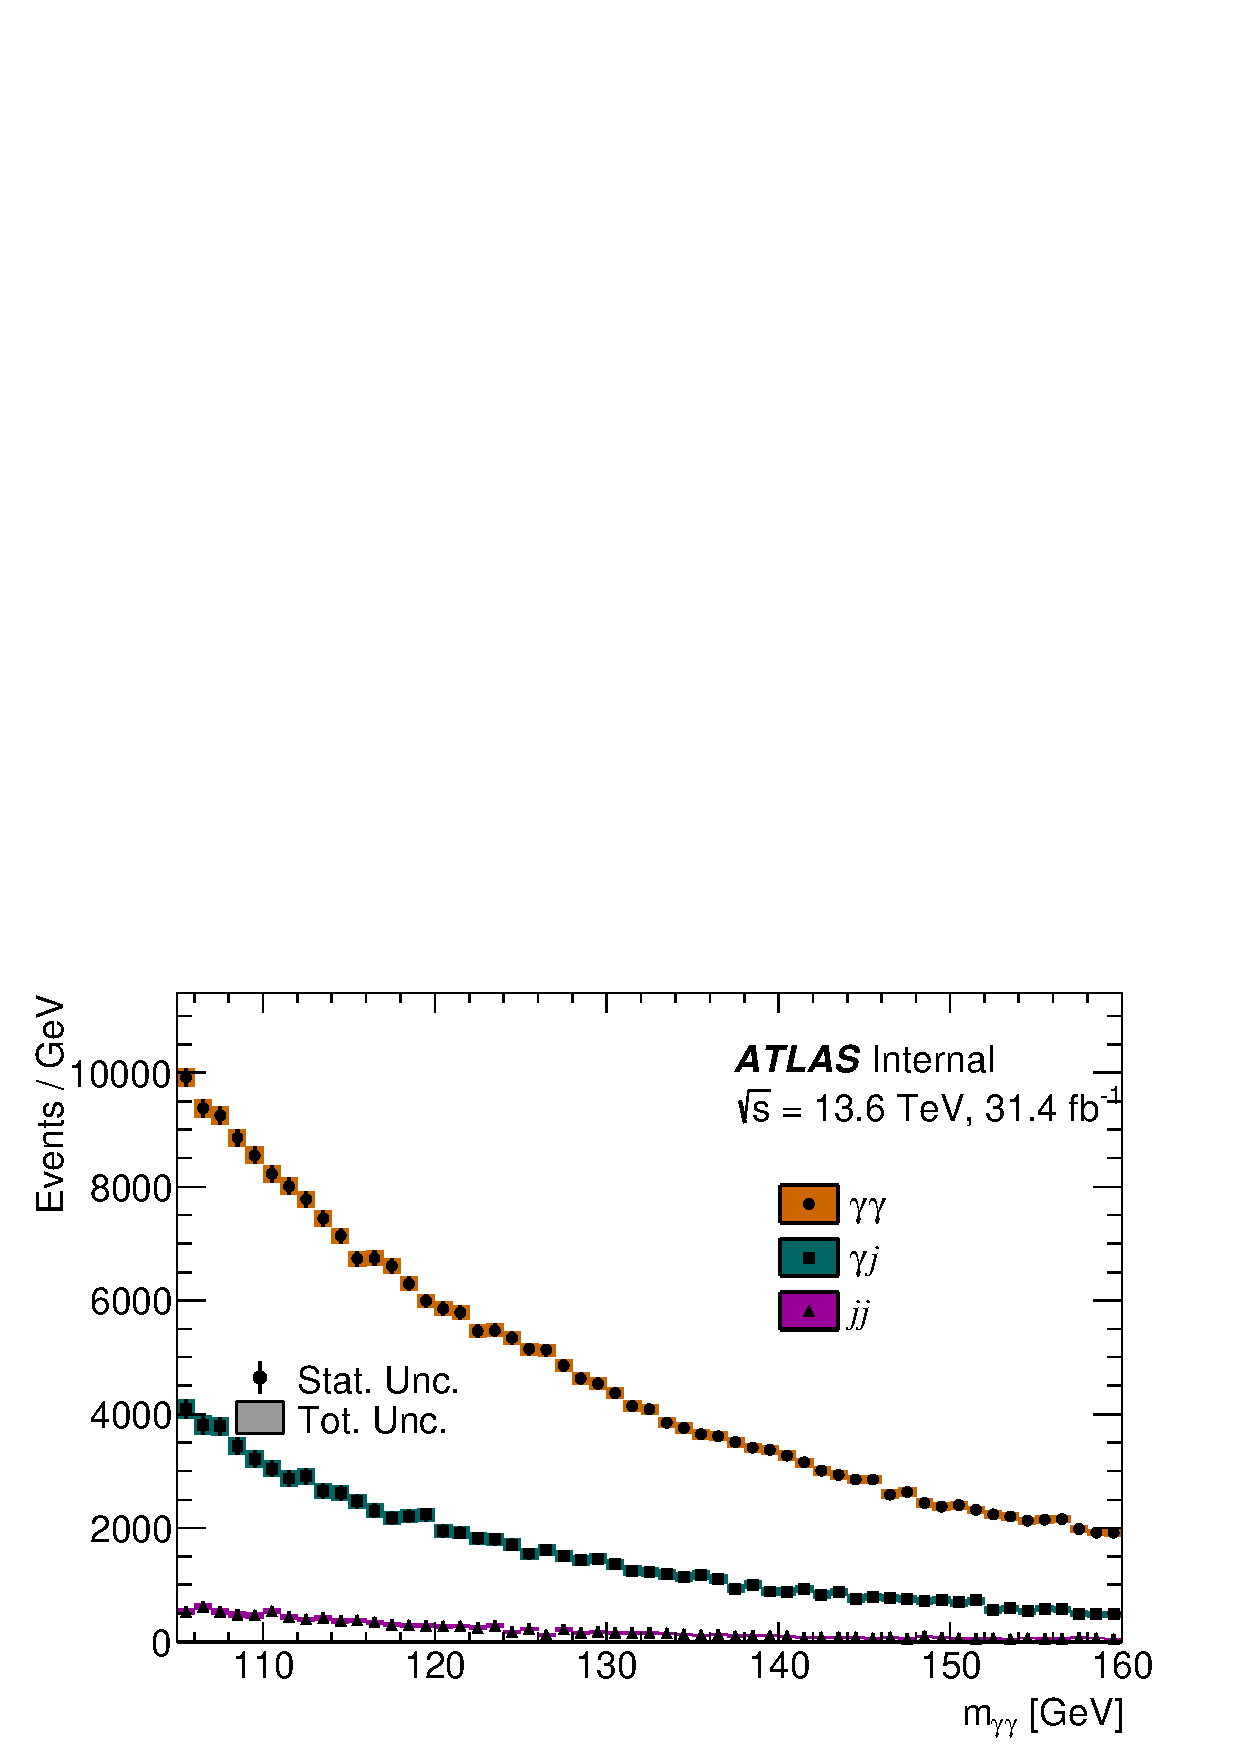
\includegraphics[width=\textwidth]{figures/2x2d_sidebands/sb_h032_2023_debug/plots/plot_bkgDecomp_Inclusive_m_yy.pdf}
%         \label{fig:2x2dmyy2023}
%     \end{subfigure}
%     \begin{subfigure}{0.45\textwidth}
%         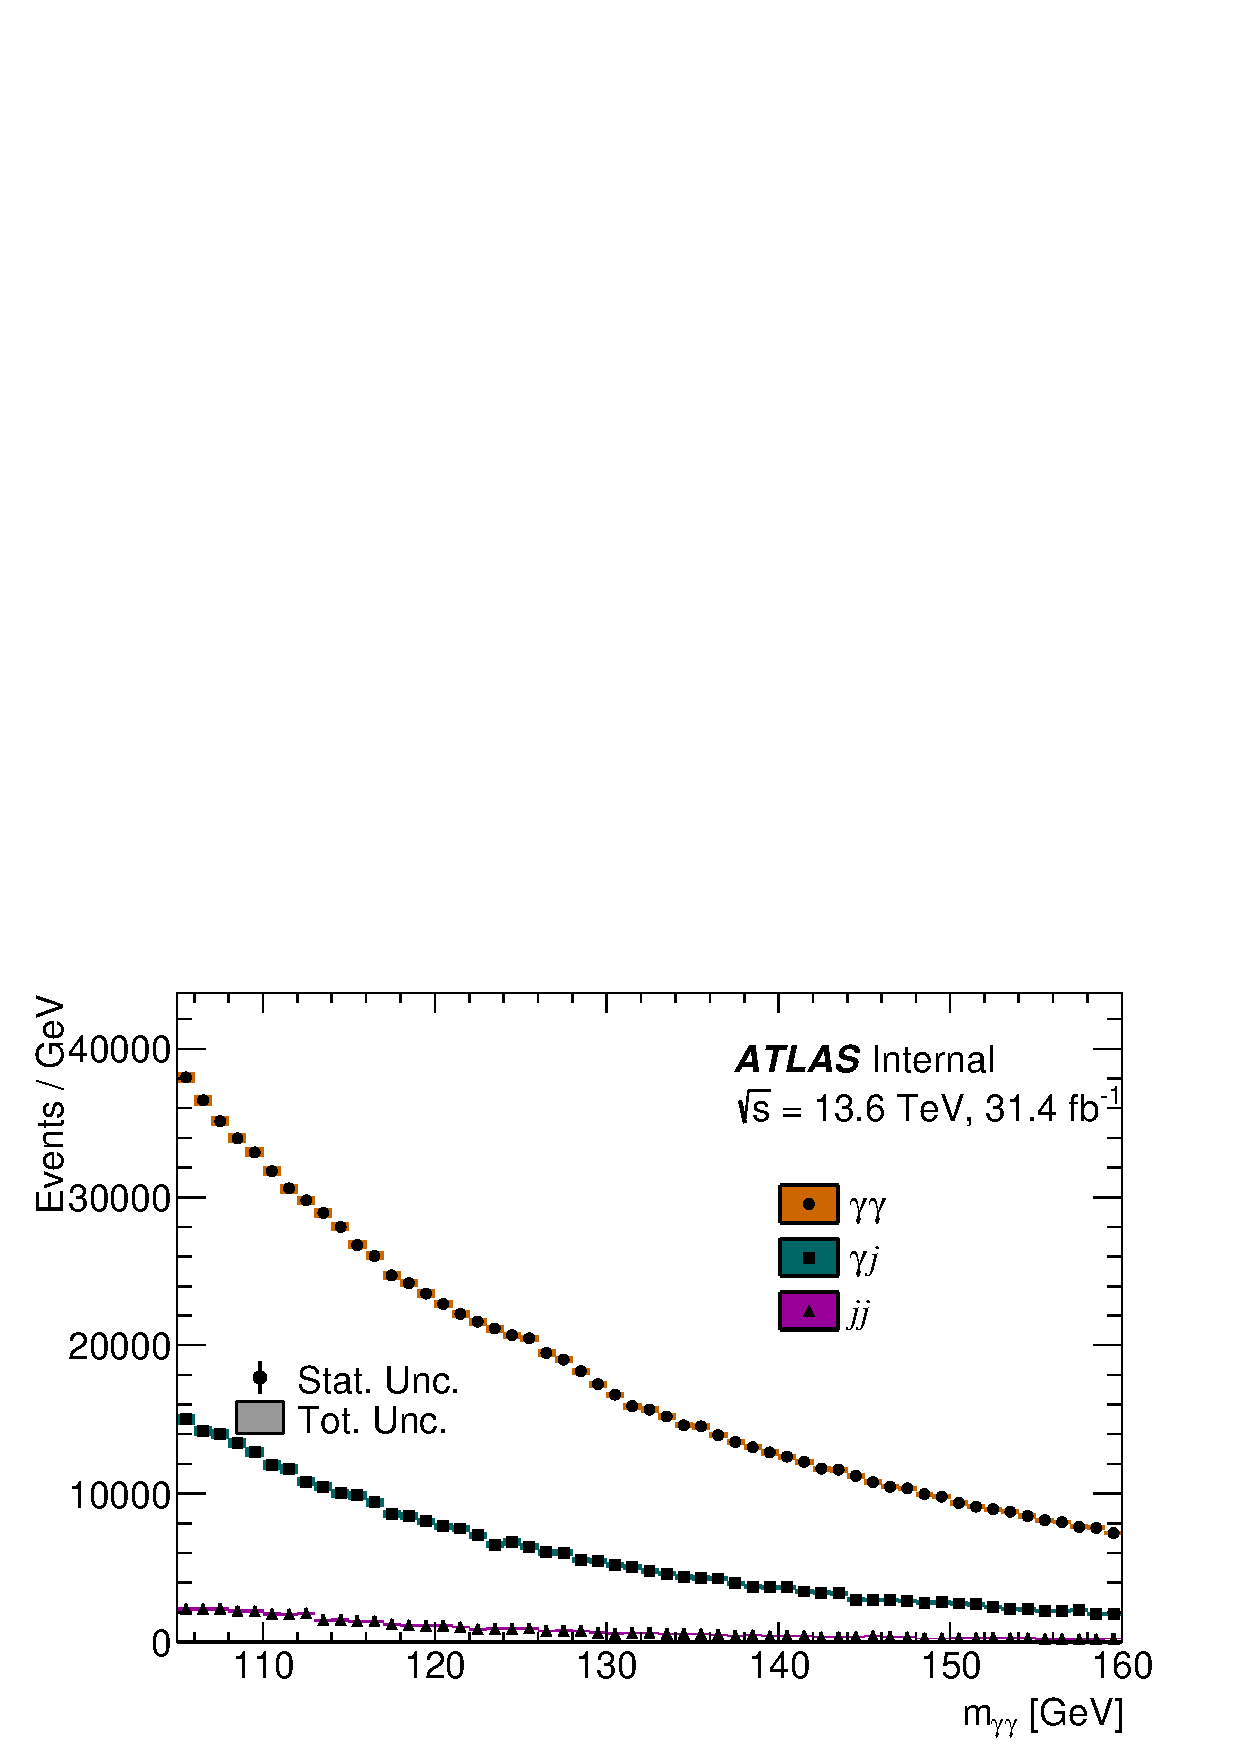
\includegraphics[width=\textwidth]{figures/2x2d_sidebands/sb_h032_2024_debug/plots/plot_bkgDecomp_Inclusive_m_yy.pdf}
%         \label{fig:2x2dmyy2024}
%     \end{subfigure}
%     \caption{Background yields as a function of $m_{\gamma \gamma}$ for 2022 (a), 2023 (b) and 2024 (c) data (\texttt{mc23a}, \texttt{mc23d} and \texttt{mc23e}).}
% \end{figure}


\begin{figure}[!h]
    \centering
    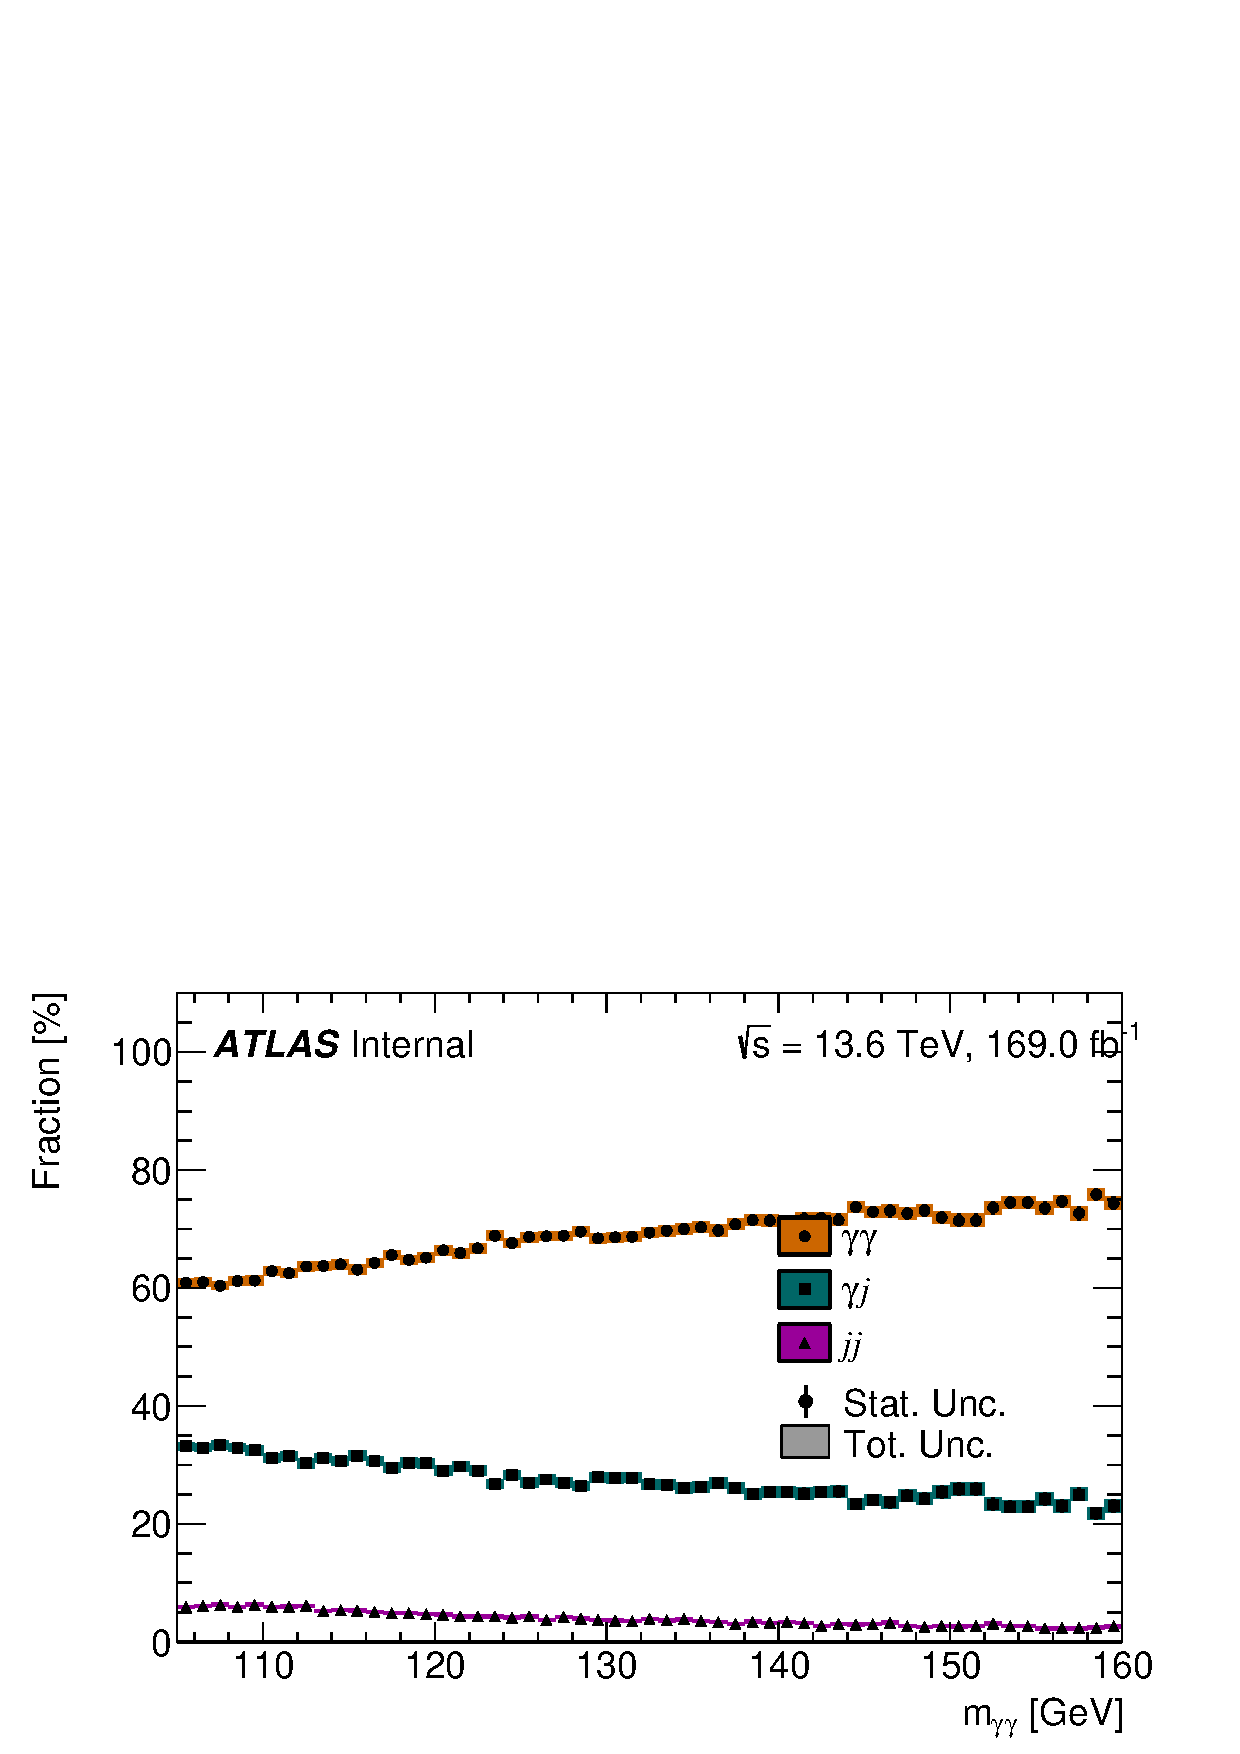
\includegraphics[width=\textwidth]{figures/2x2d_sidebands/sb_out_2022-24/plots/plot_purity_m_yy.pdf}
    \label{fig:2x2dpurmyy202224}
    \caption{Background purity as a function of $m_{\gamma \gamma}$ for 2022--2024 data (\texttt{mc23a--e}).}
\end{figure}

% \begin{figure}[!h]
%     \centering
%     \begin{subfigure}{0.45\textwidth}
%         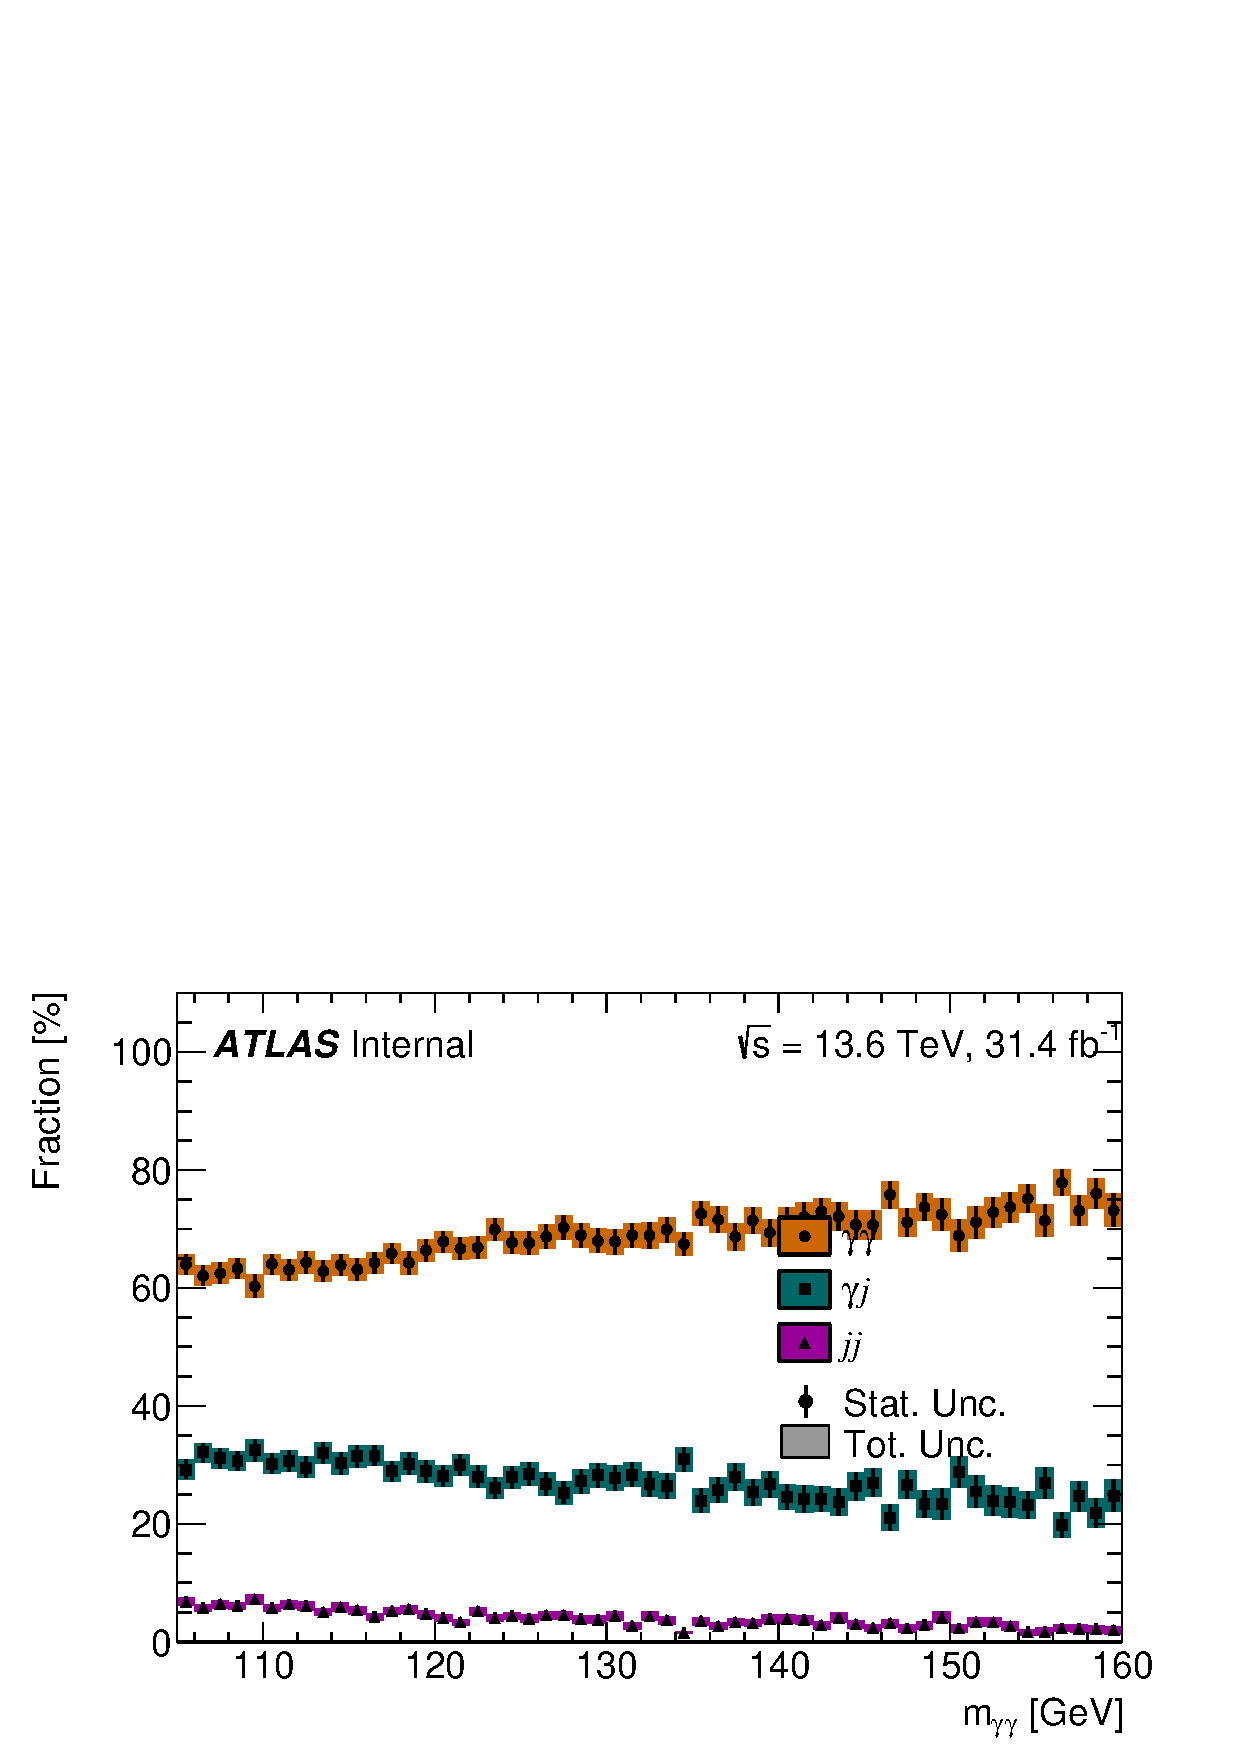
\includegraphics[width=\textwidth]{figures/2x2d_sidebands/sb_h032_2022_debug/plots/plot_purity_m_yy.pdf}
%         \label{fig:2x2dpurmyy2022}
%     \end{subfigure}
%     \begin{subfigure}{0.45\textwidth}
%         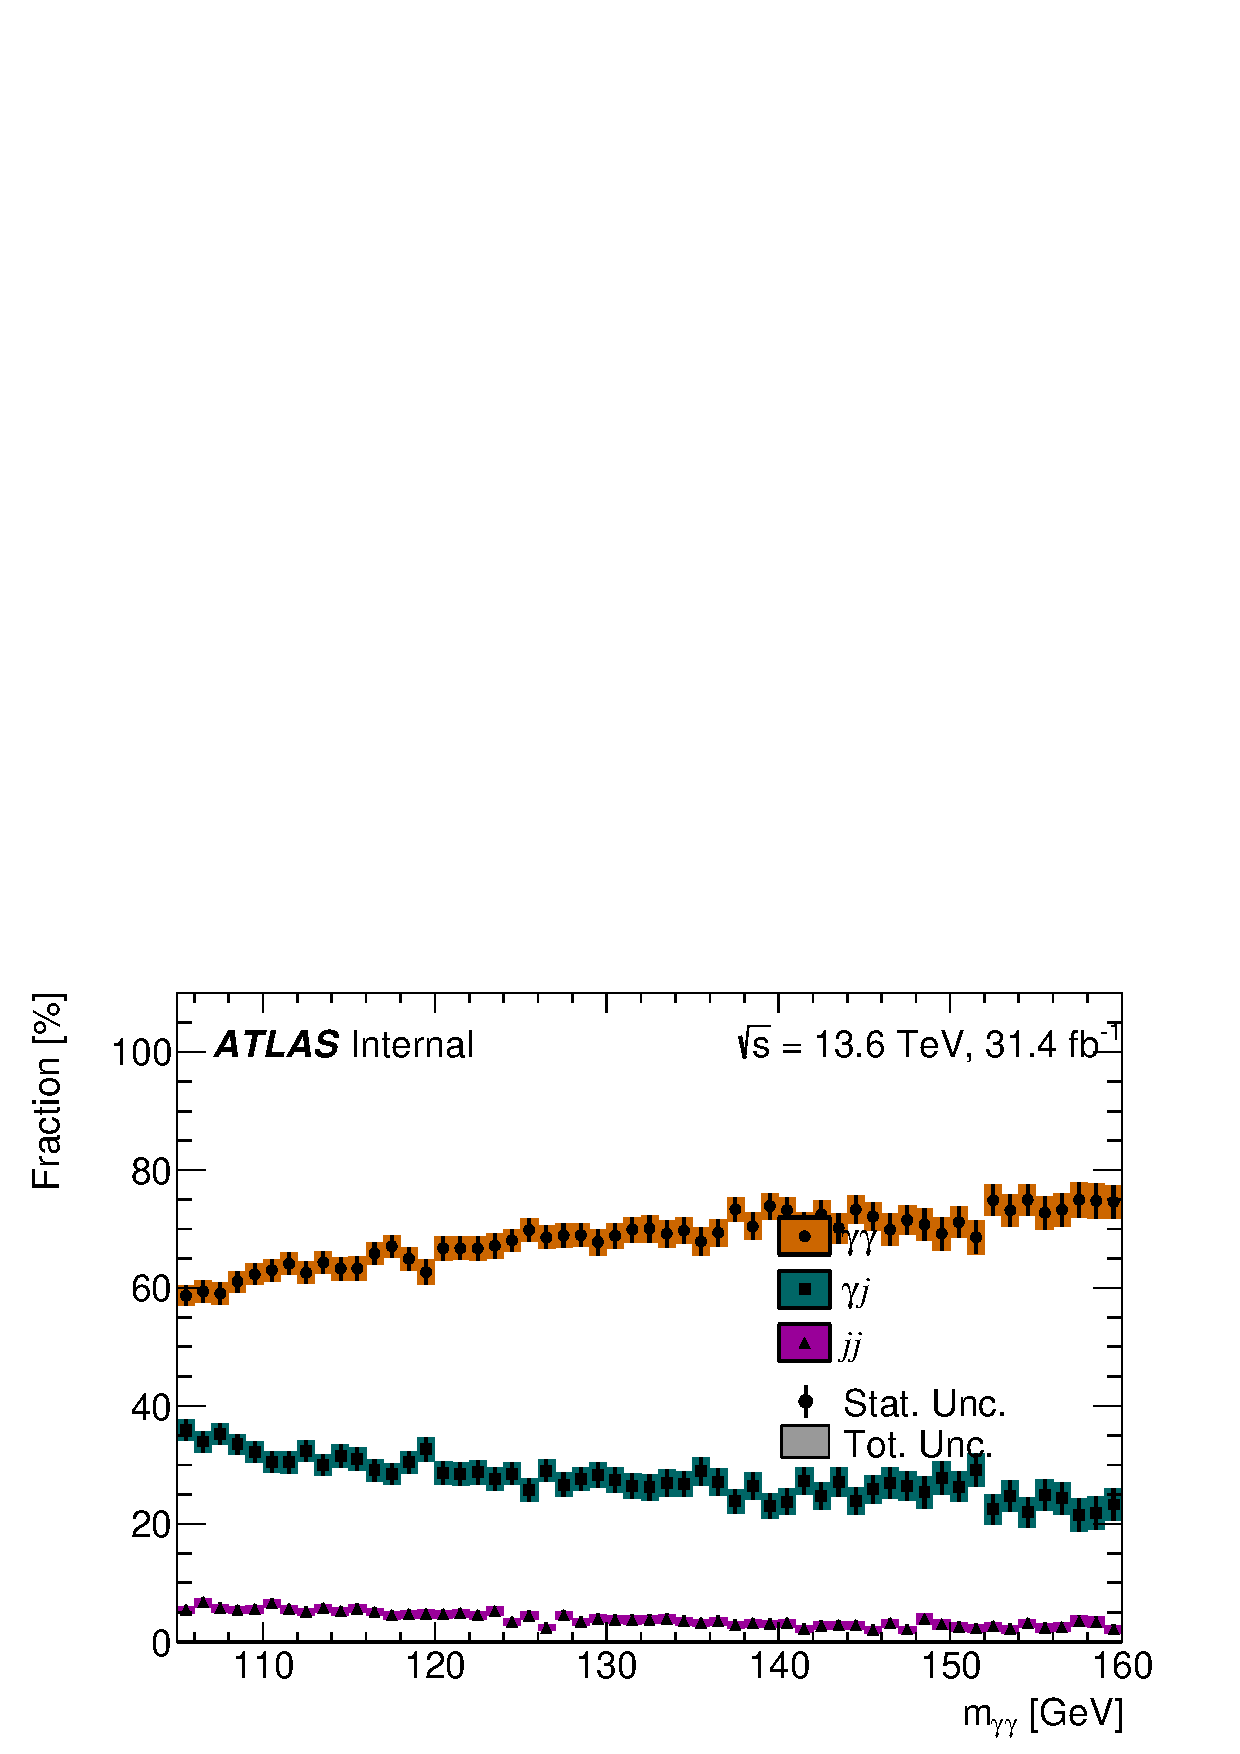
\includegraphics[width=\textwidth]{figures/2x2d_sidebands/sb_h032_2023_debug/plots/plot_purity_m_yy.pdf}
%         \label{fig:2x2dpurmyy2023}
%     \end{subfigure}
%     \begin{subfigure}{0.45\textwidth}
%         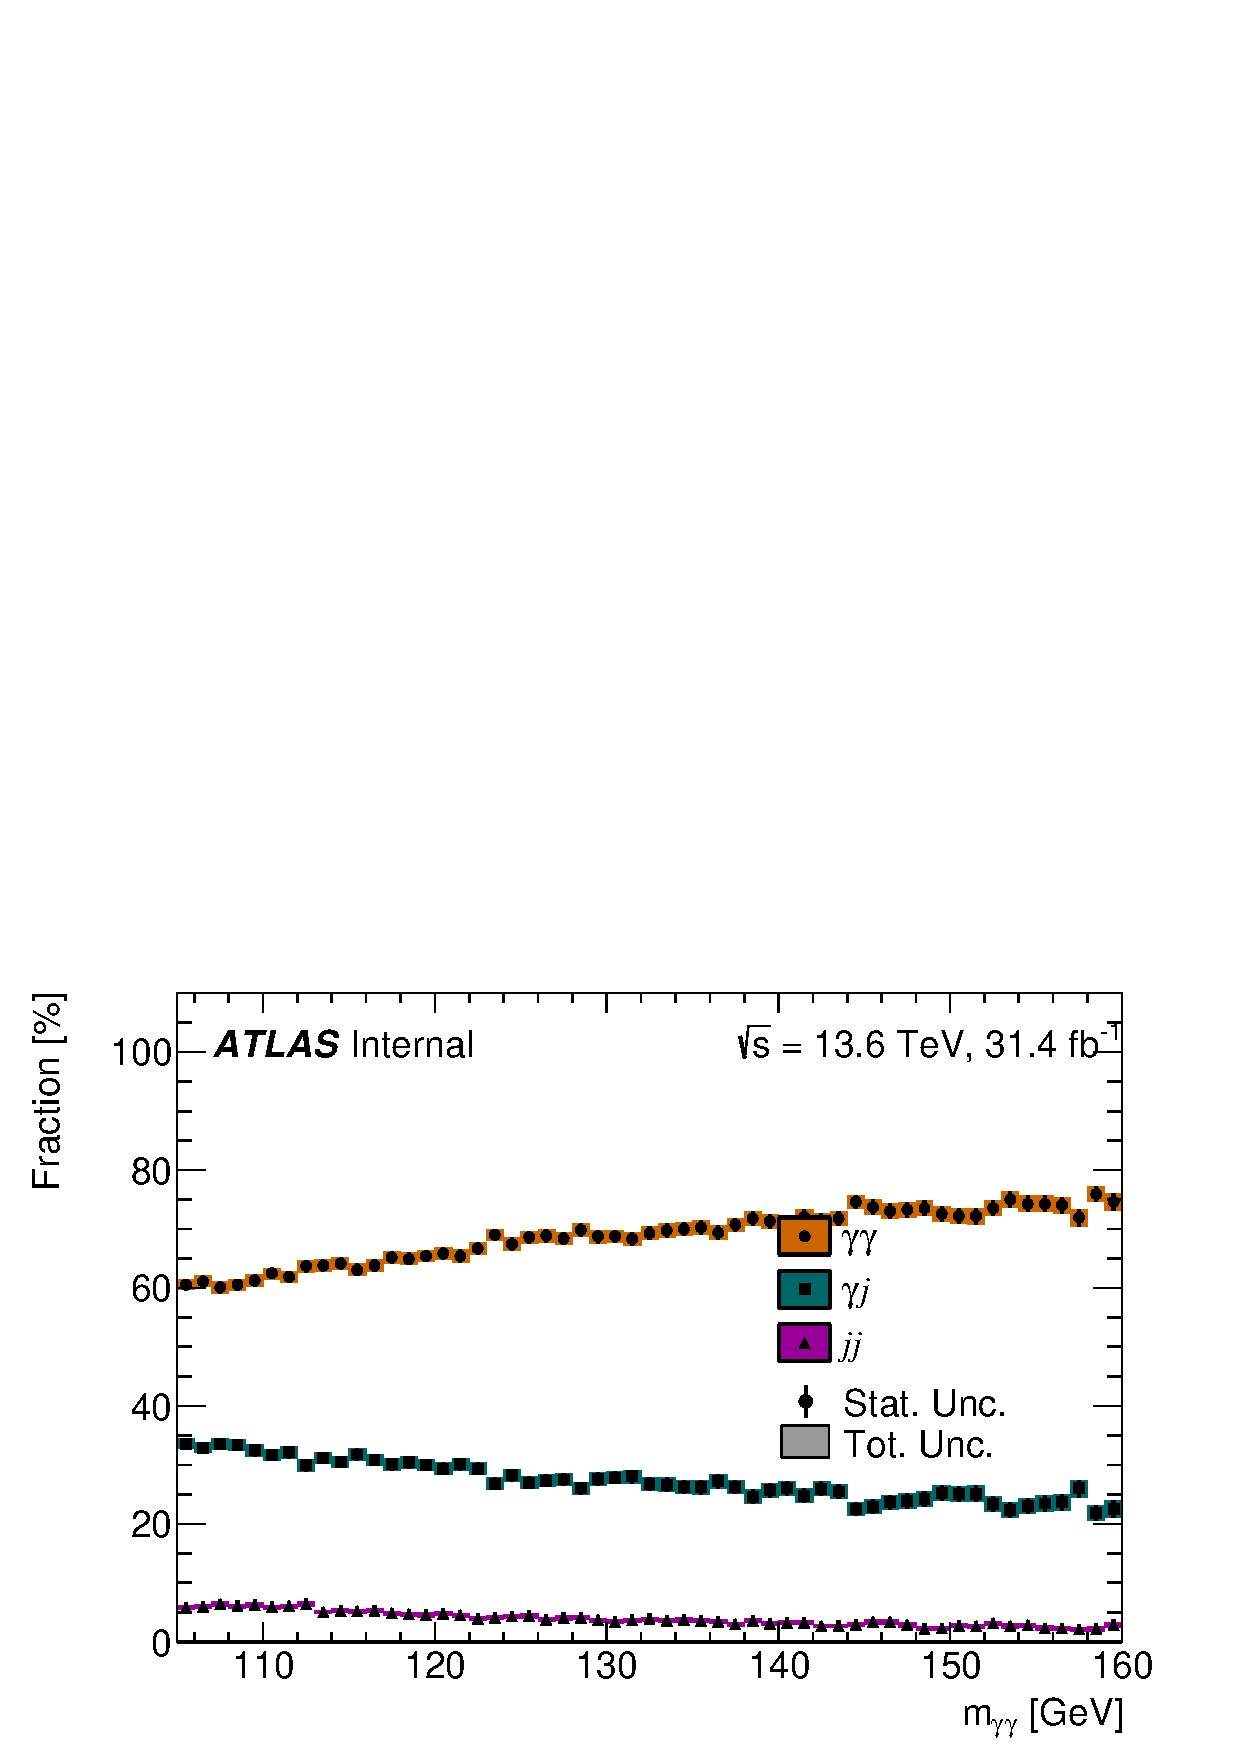
\includegraphics[width=\textwidth]{figures/2x2d_sidebands/sb_h032_2024_debug/plots/plot_purity_m_yy.pdf}
%         \label{fig:2x2dpurmyy2024}
%     \end{subfigure}
%     \caption{Background purity vs. $m_{\gamma \gamma}$ for 2022 (a), 2023 (b) and 2024 (c) data (\texttt{mc23a}, \texttt{mc23d} and \texttt{mc23e}).}
% \end{figure}

\begin{figure}[!h]
    \centering
    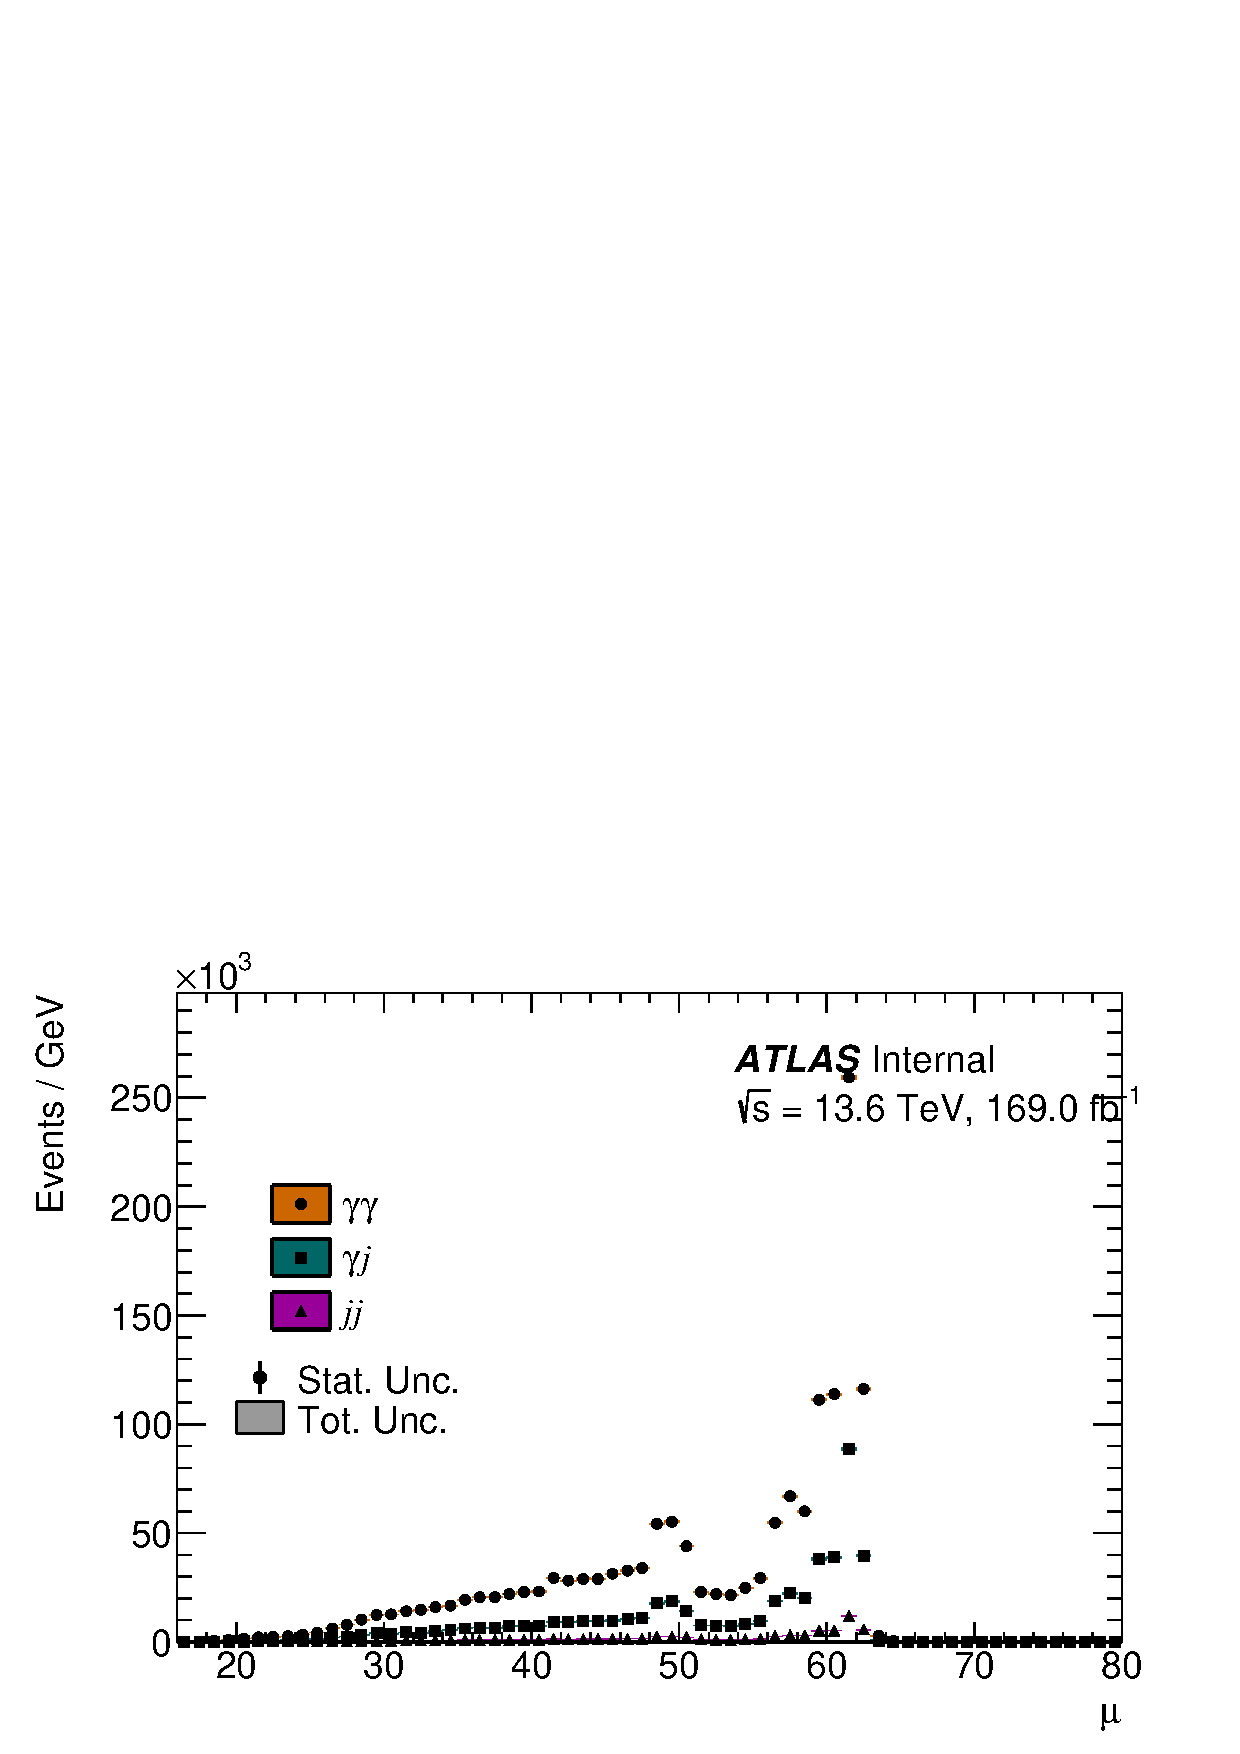
\includegraphics[width=\textwidth]{figures/2x2d_sidebands/sb_out_2022-24/plots/plot_bkgDecomp_Inclusive_mu.pdf}
    \label{fig:2x2dmu202224}
    \caption{Background yields as a function of $\mu$ for 2022--2024 data (\texttt{mc23a--e}).}
\end{figure}


% \begin{figure}[!h]
%     \centering
%     \begin{subfigure}{0.45\textwidth}
%         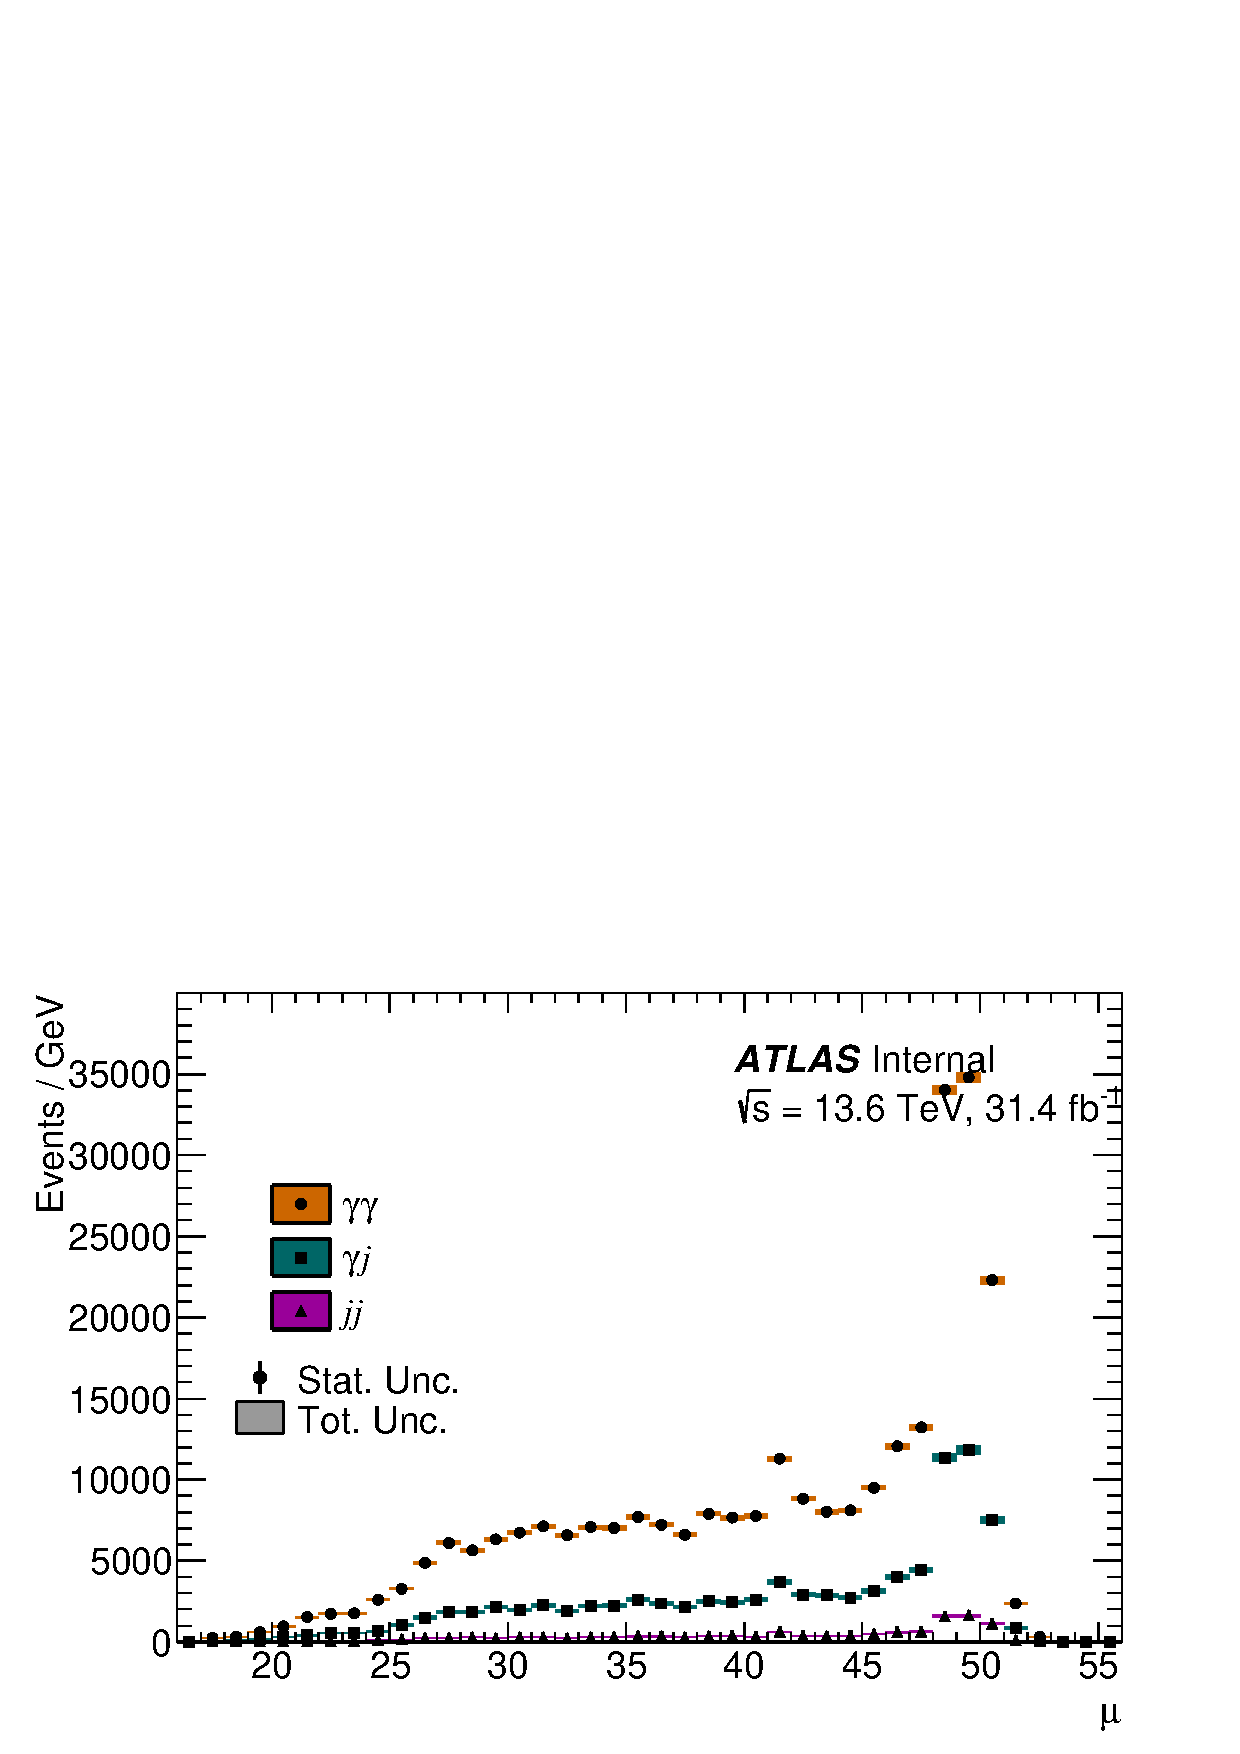
\includegraphics[width=\textwidth]{figures/2x2d_sidebands/sb_h032_2022_debug/plots/plot_bkgDecomp_Inclusive_mu.pdf}
%         \label{fig:2x2dmu2022}
%     \end{subfigure}
%     \begin{subfigure}{0.45\textwidth}
%         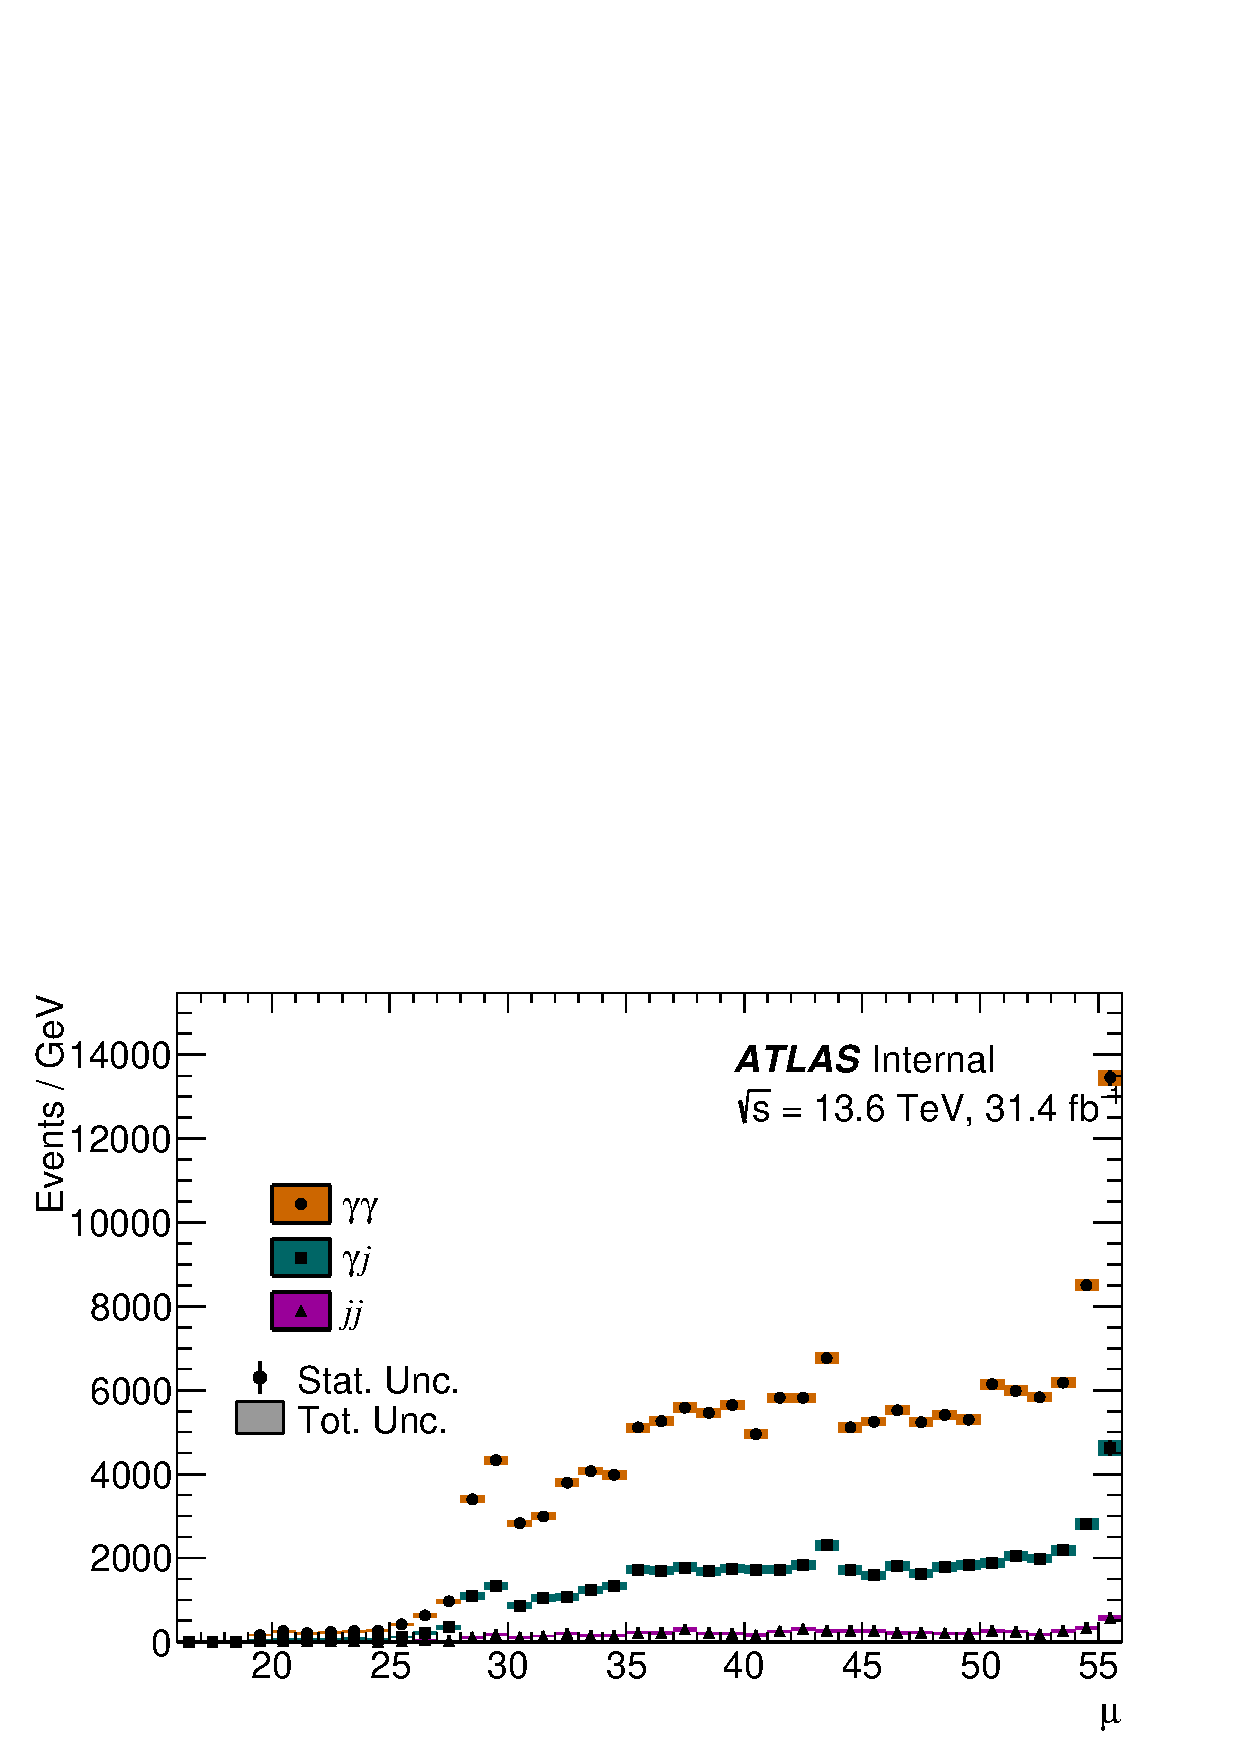
\includegraphics[width=\textwidth]{figures/2x2d_sidebands/sb_h032_2023_debug/plots/plot_bkgDecomp_Inclusive_mu.pdf}
%         \label{fig:2x2dmu2023}
%     \end{subfigure}
%     \begin{subfigure}{0.45\textwidth}
%         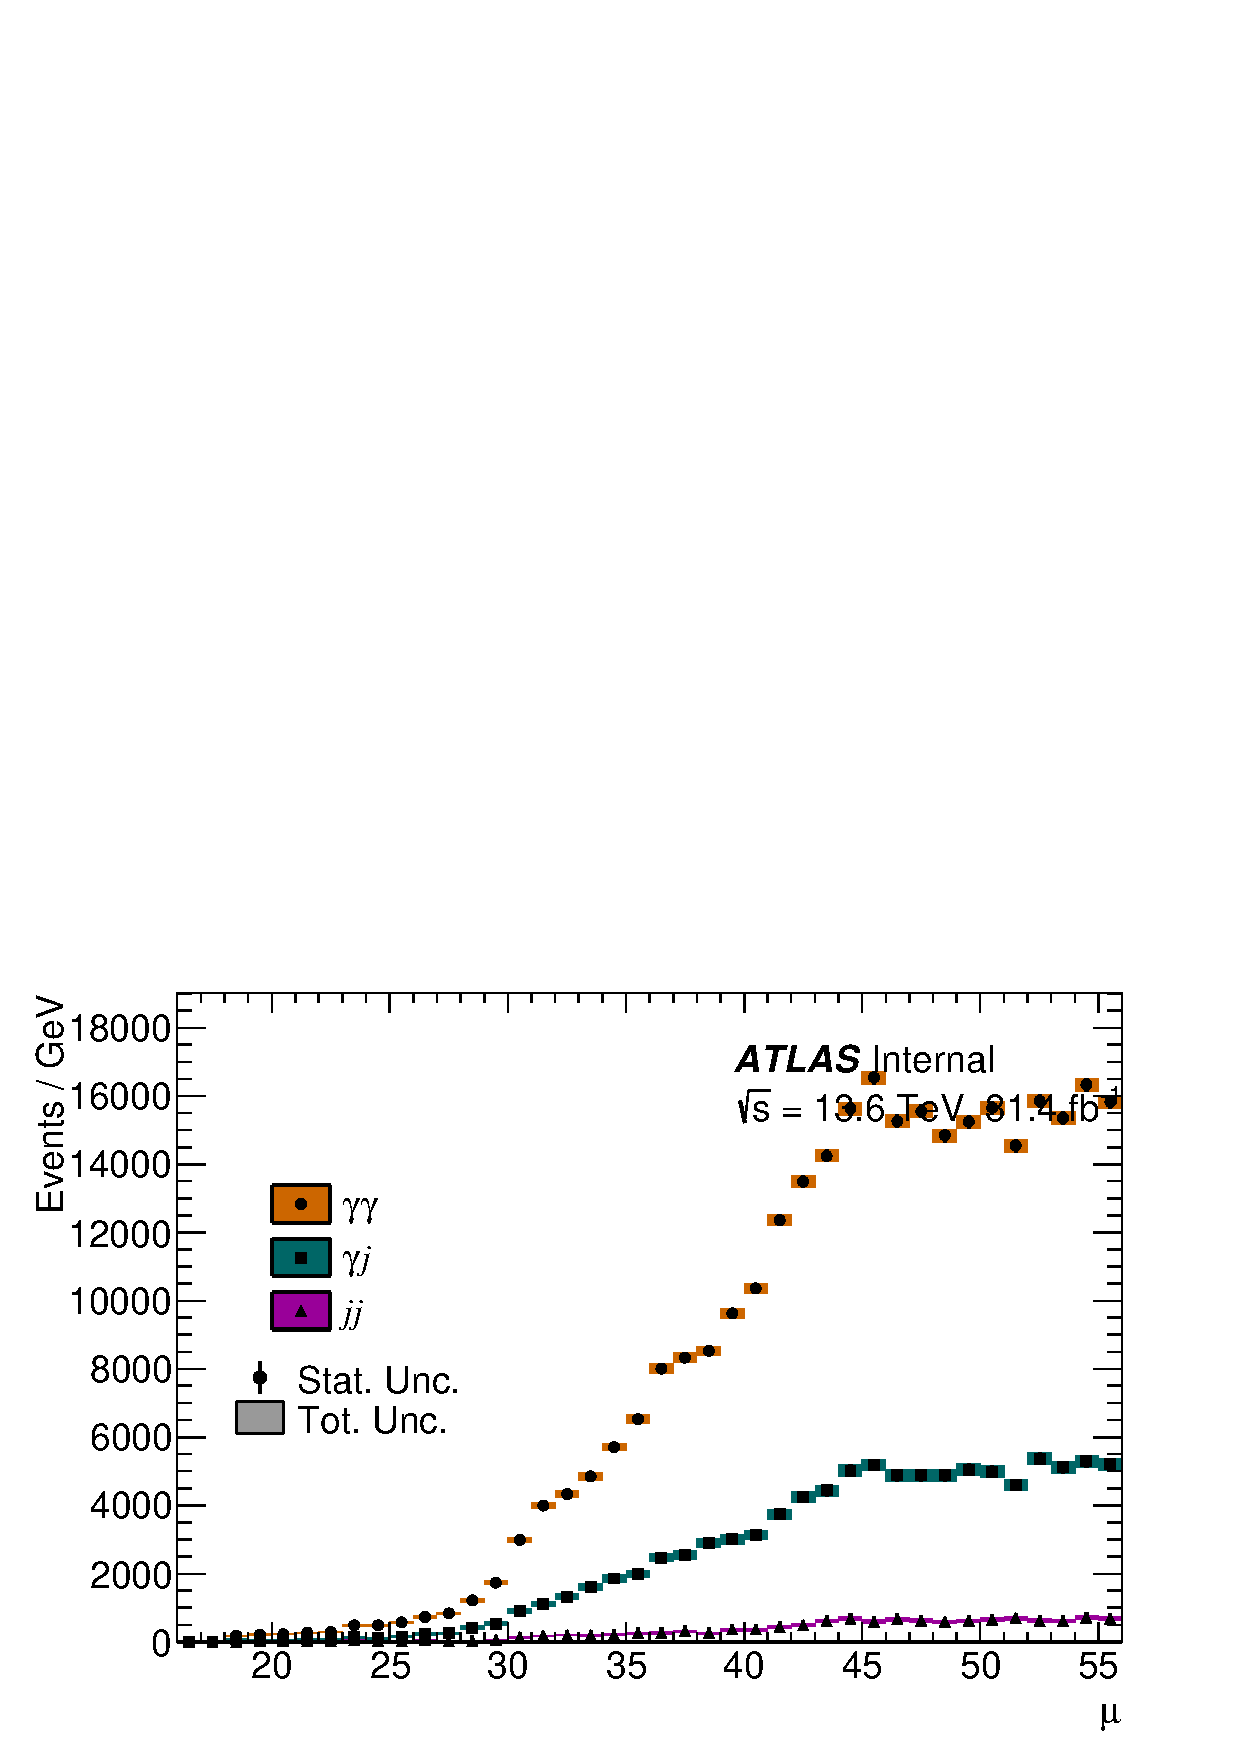
\includegraphics[width=\textwidth]{figures/2x2d_sidebands/sb_h032_2024_debug/plots/plot_bkgDecomp_Inclusive_mu.pdf}
%         \label{fig:2x2dmu2024}
%     \end{subfigure}
%     \caption{Background yields as a function of $\mu$ for 2022 (a), 2023 (b) and 2024 (c) data (\texttt{mc23a}, \texttt{mc23d} and \texttt{mc23e}).}
% \end{figure}

\begin{figure}[!h]
    \centering
    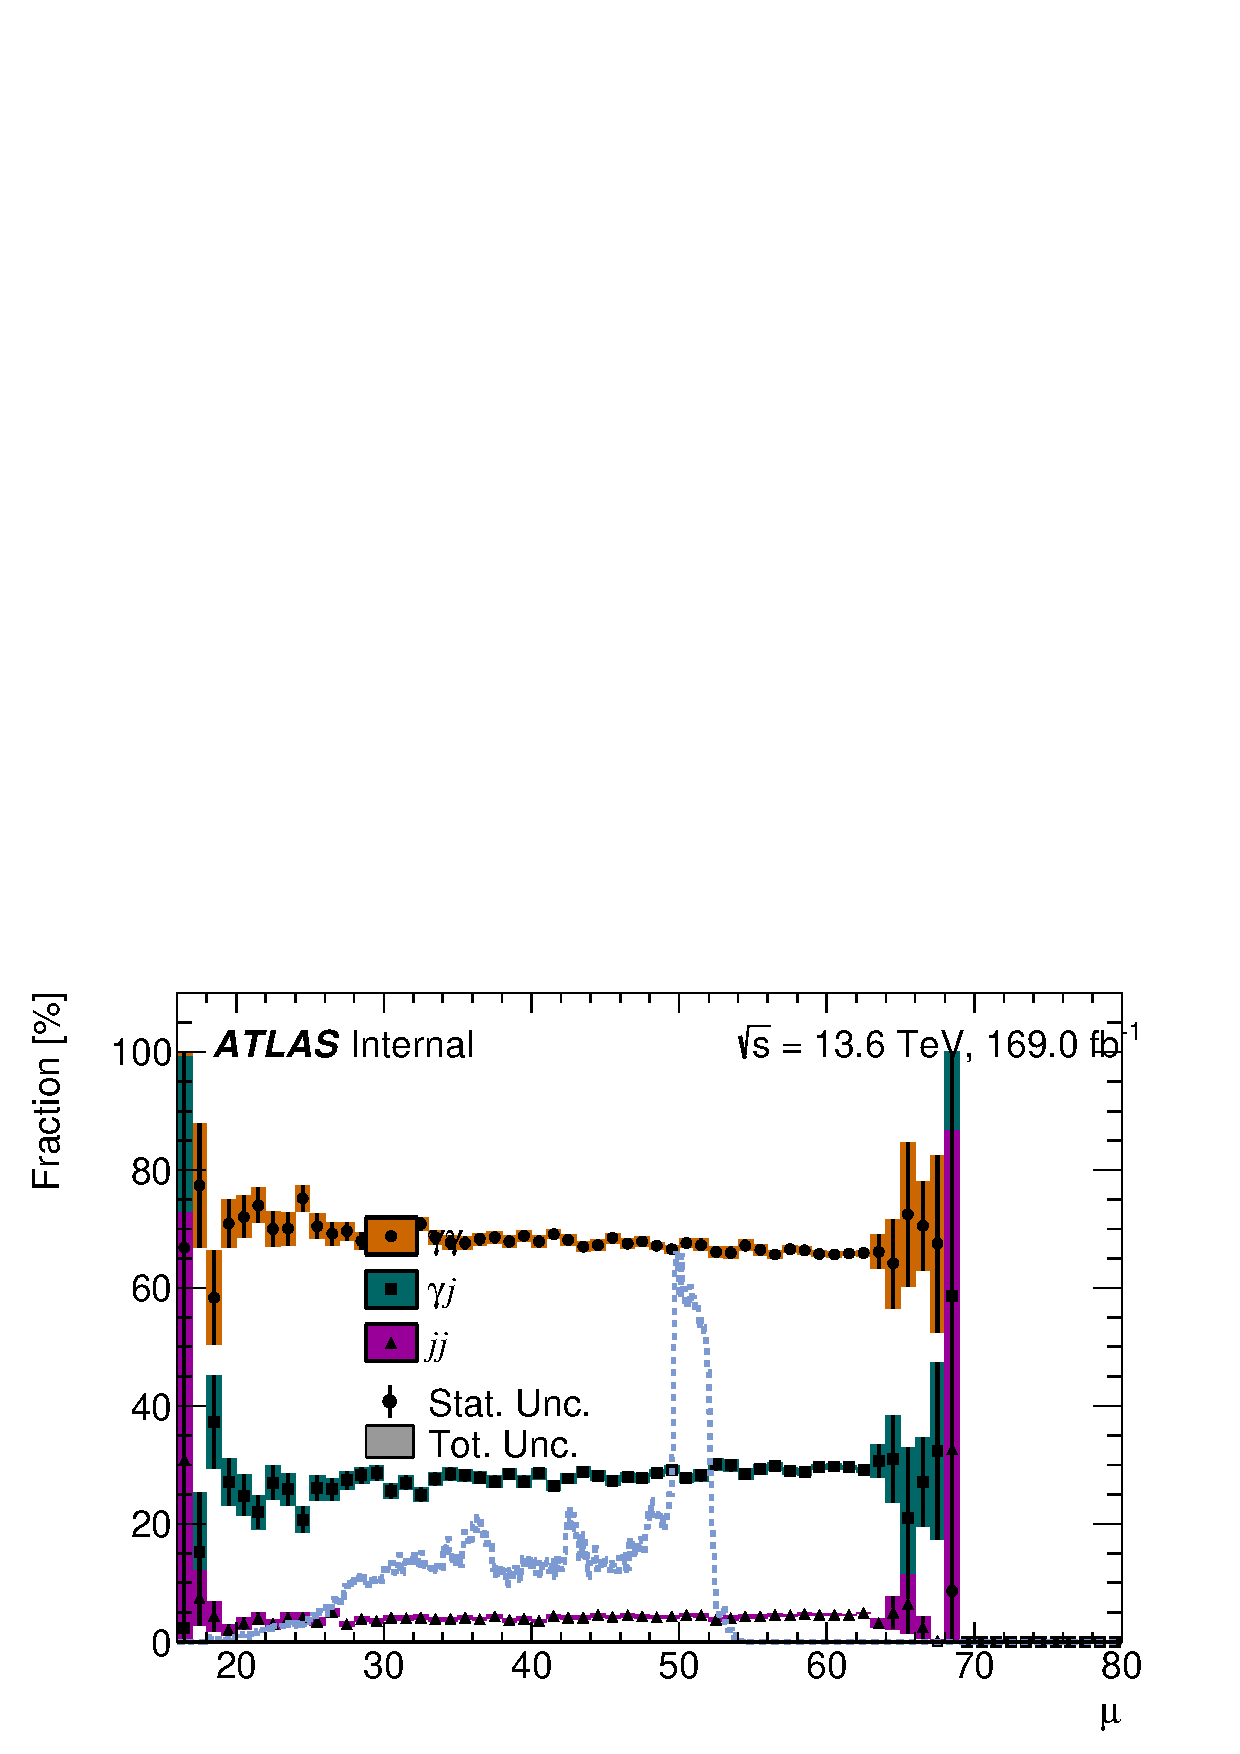
\includegraphics[width=\textwidth]{figures/2x2d_sidebands/sb_out_2022-24/plots/plot_purity_mu.pdf}
    \label{fig:2x2dpurmu202224}
    \caption{Background purity as a function of $\mu$ for 2022--2024 data (\texttt{mc23a--e}).}
\end{figure}


% \begin{figure}[!h]
%     \centering
%     \begin{subfigure}{0.45\textwidth}
%         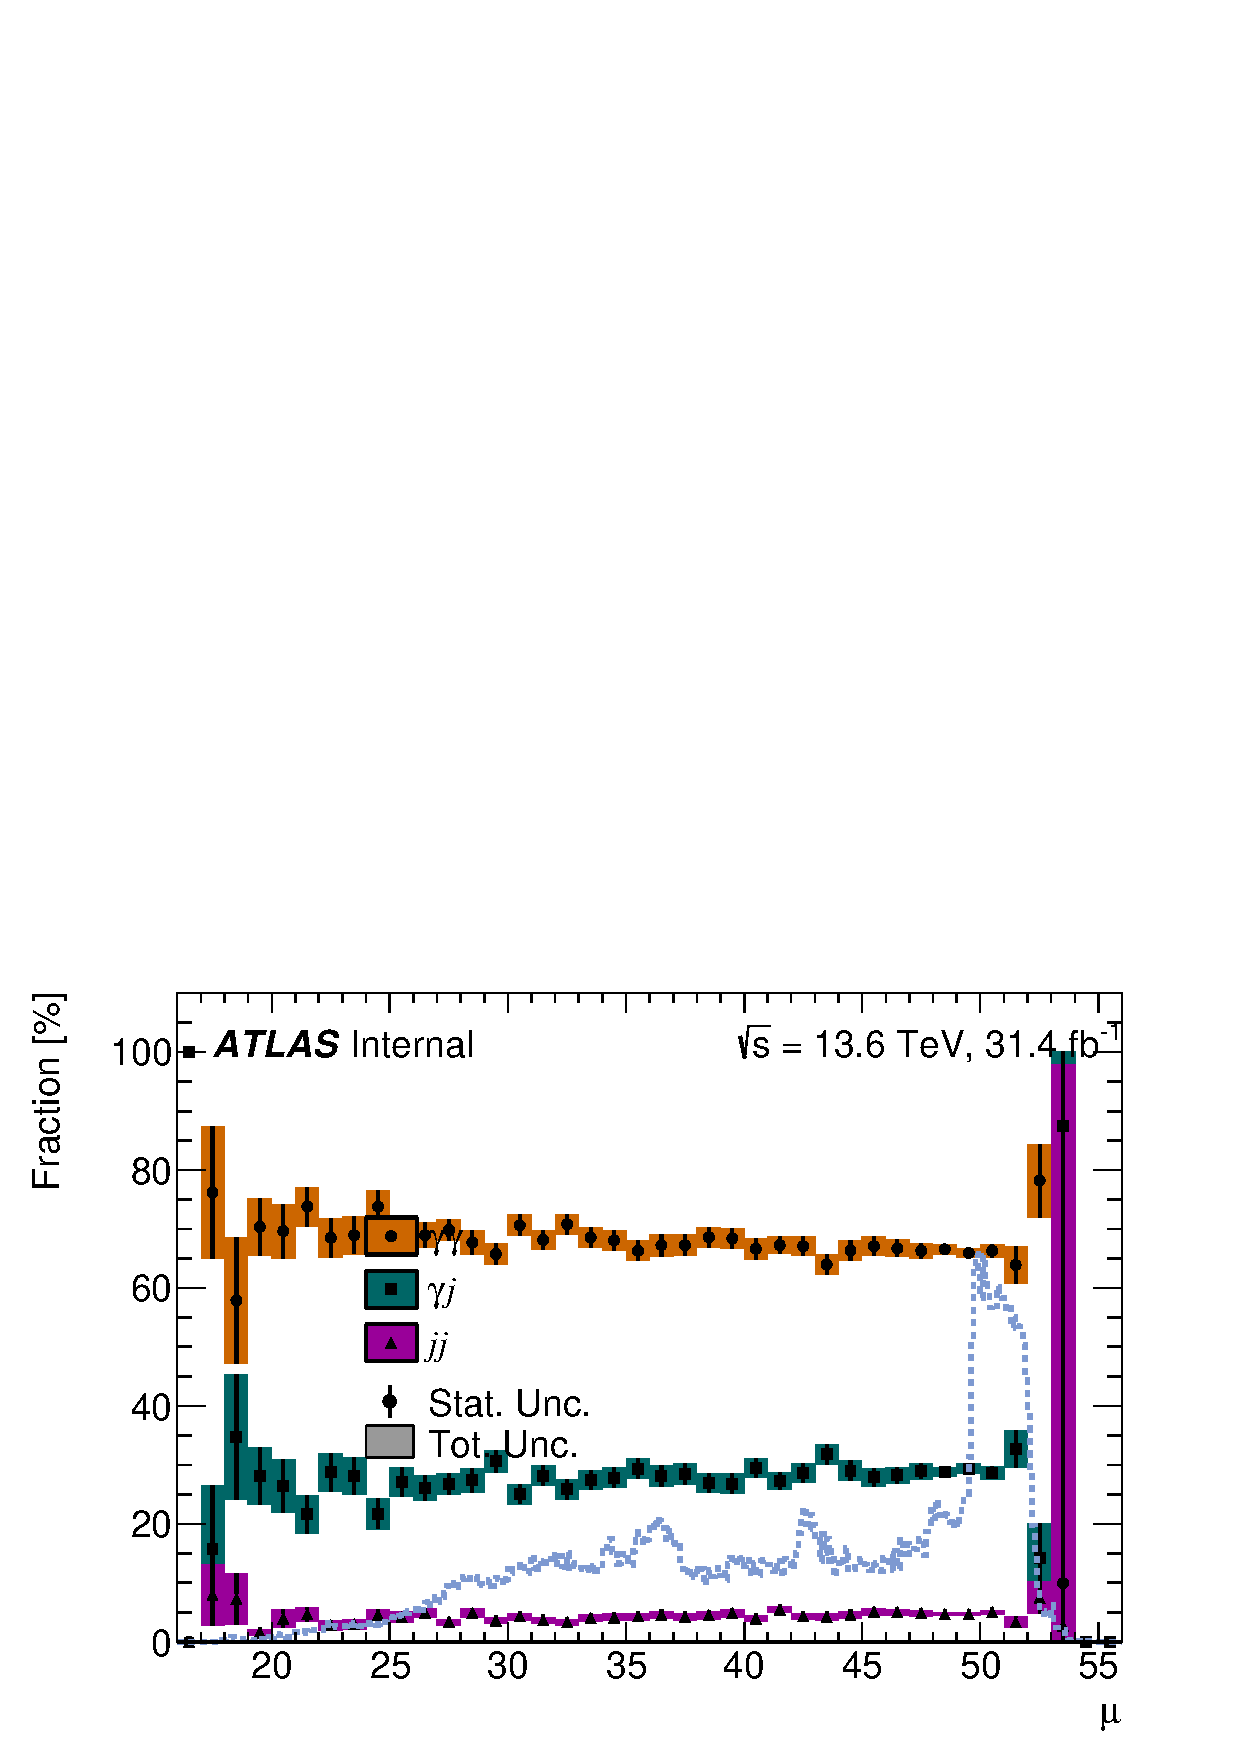
\includegraphics[width=\textwidth]{figures/2x2d_sidebands/sb_h032_2022_debug/plots/plot_purity_mu.pdf}
%         \label{fig:2x2dpurmu2022}
%     \end{subfigure}
%     \begin{subfigure}{0.45\textwidth}
%         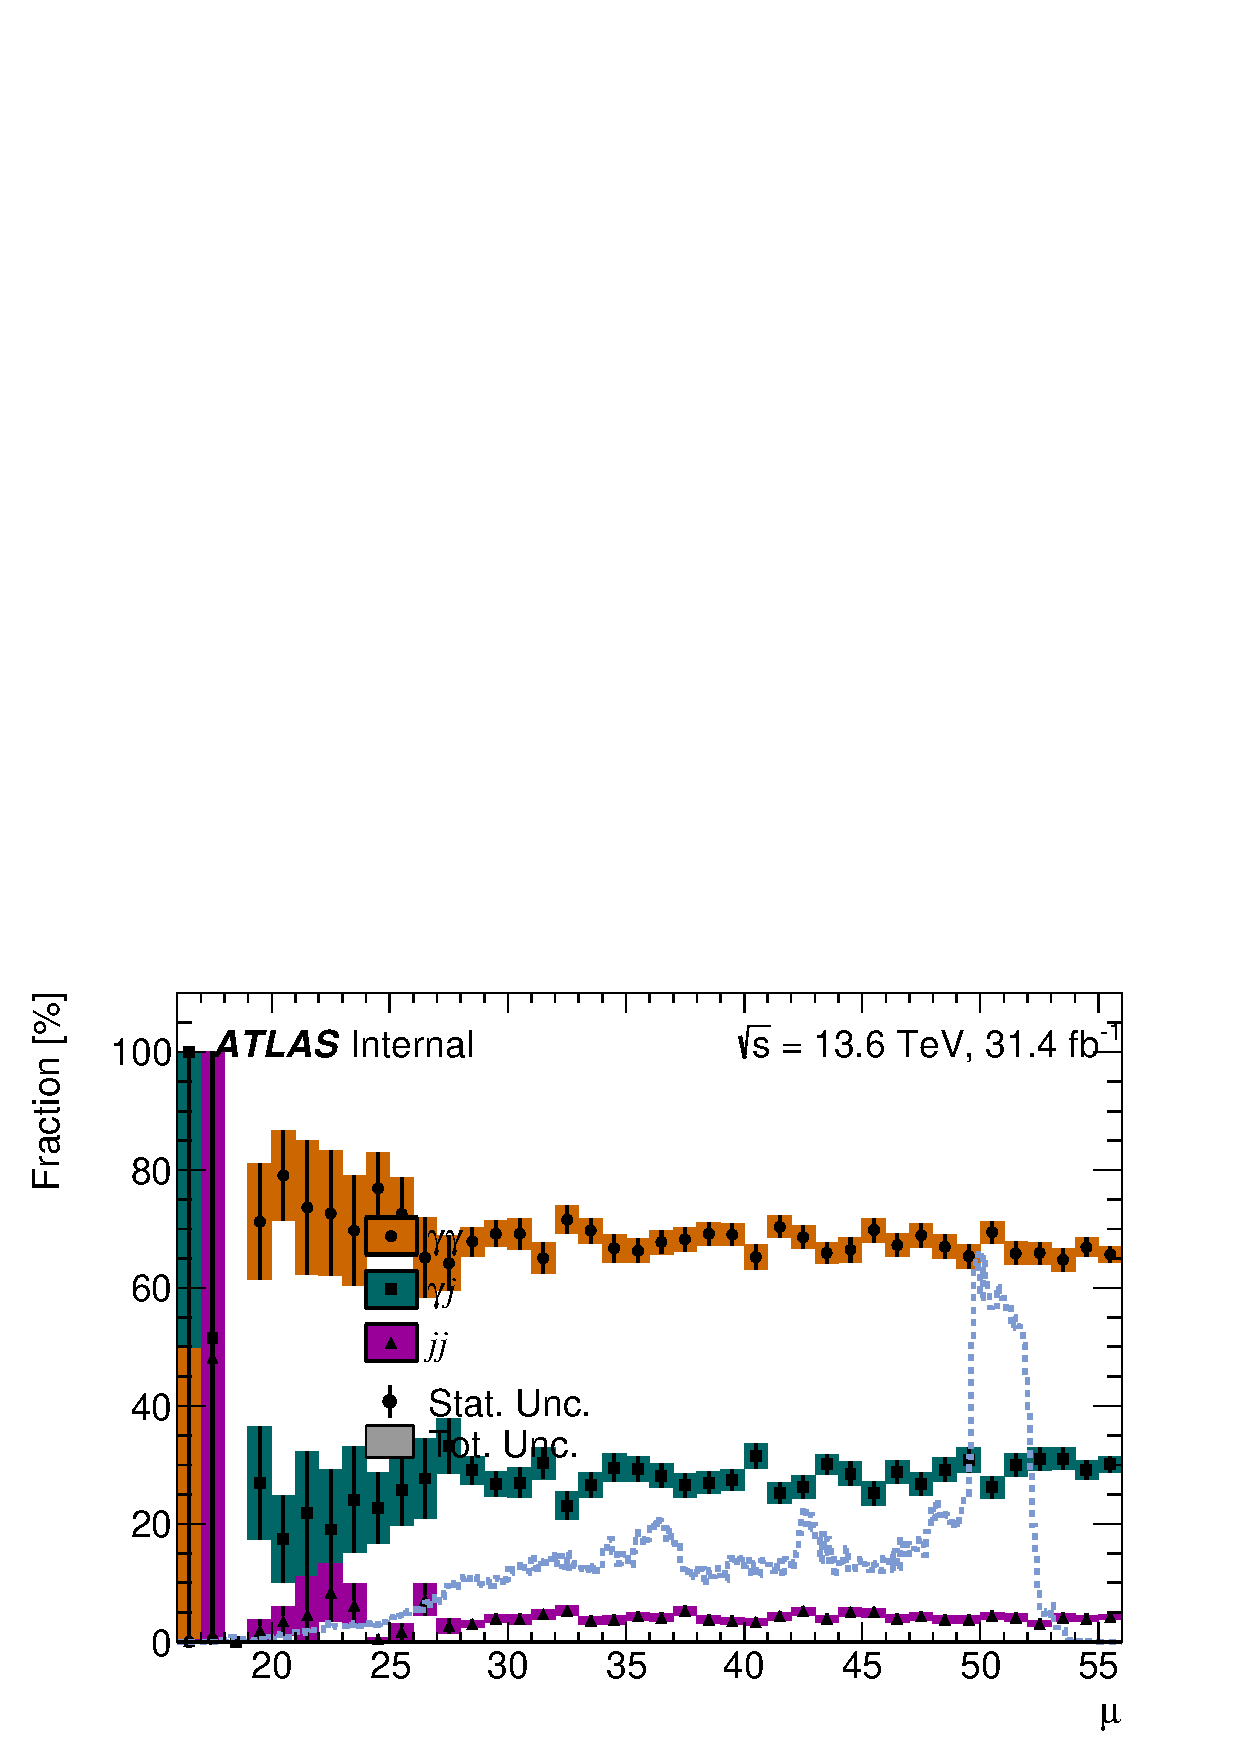
\includegraphics[width=\textwidth]{figures/2x2d_sidebands/sb_h032_2023_debug/plots/plot_purity_mu.pdf}
%         \label{fig:2x2dpurmu2023}
%     \end{subfigure}
%     \begin{subfigure}{0.45\textwidth}
%         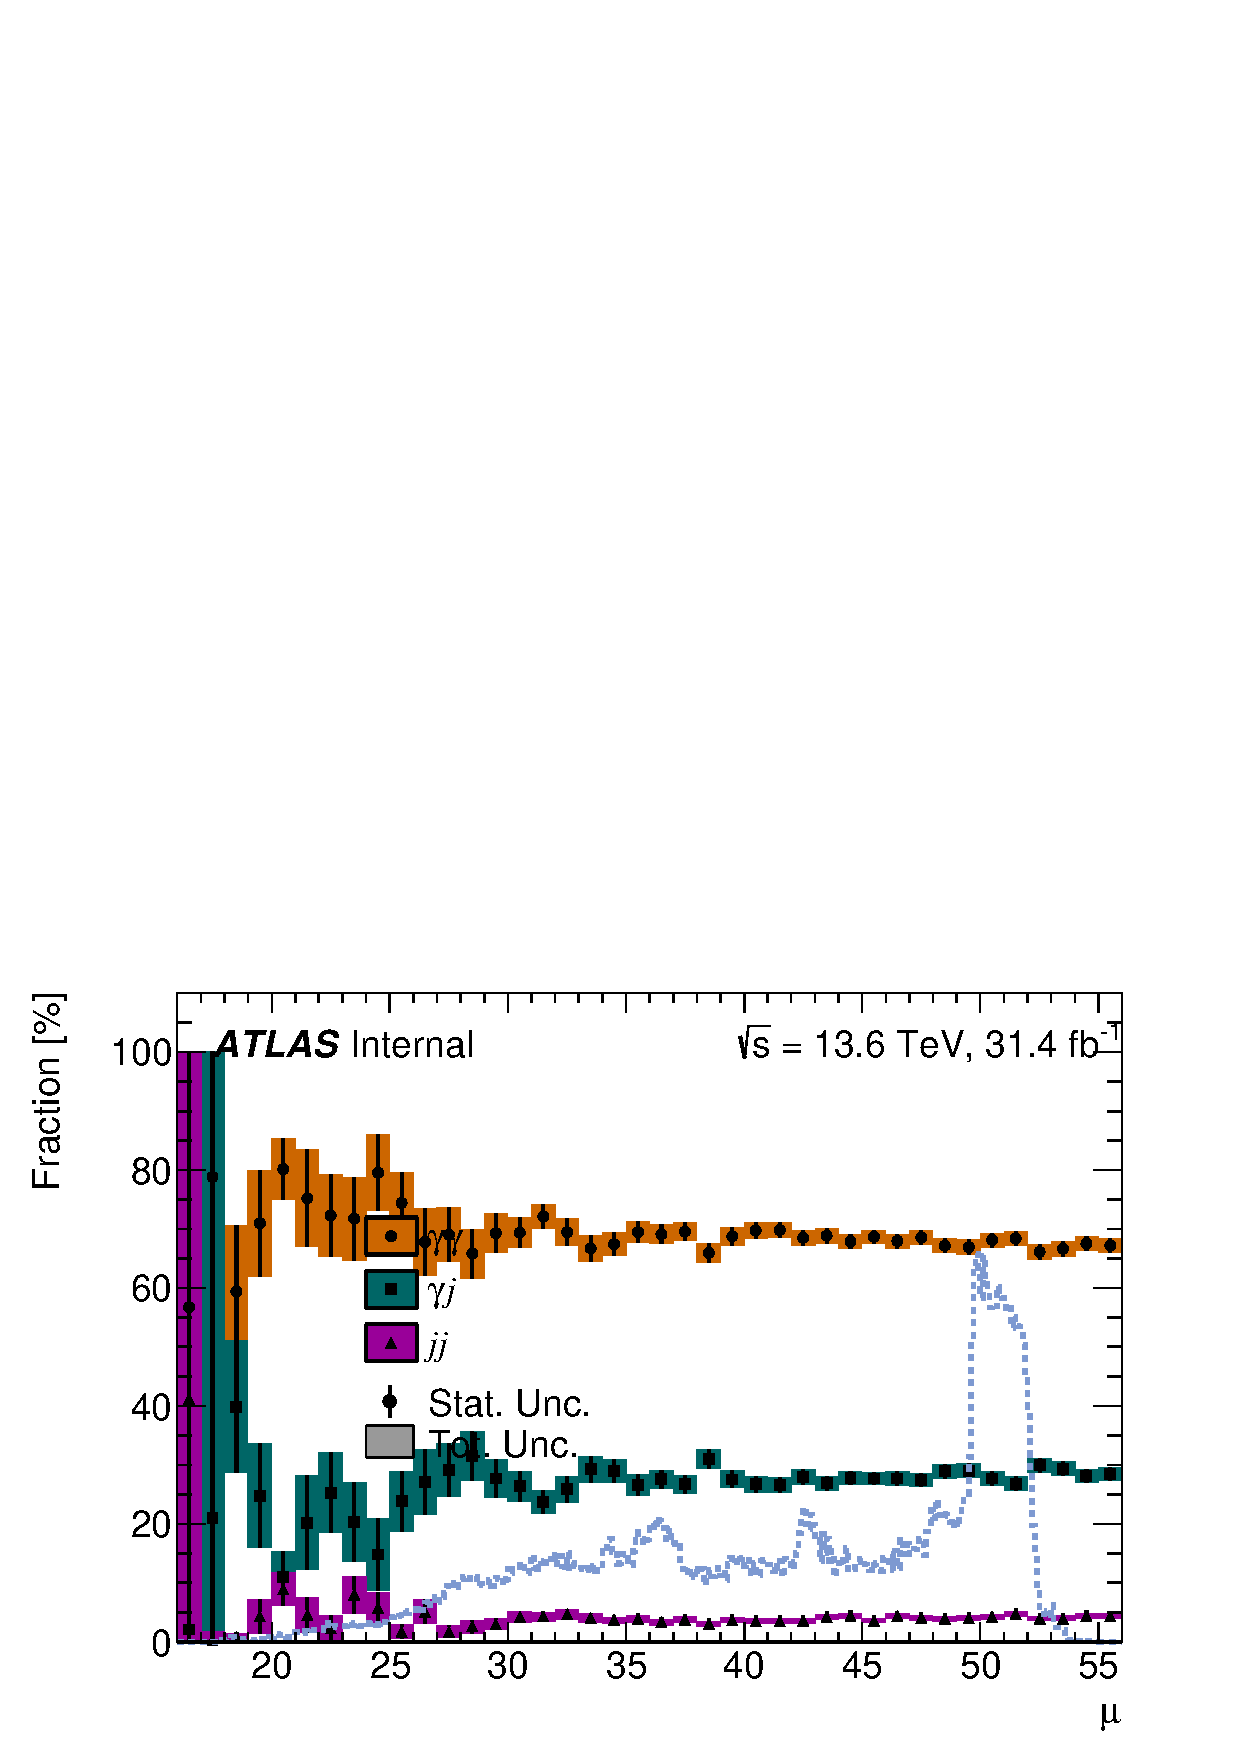
\includegraphics[width=\textwidth]{figures/2x2d_sidebands/sb_h032_2024_debug/plots/plot_purity_mu.pdf}
%         \label{fig:2x2dpurmu2024}
%     \end{subfigure}
%     \caption{Background purity vs. $\mu$ for 2022 (a), 2023 (b) and 2024 (c) data (\texttt{mc23a}, \texttt{mc23d} and \texttt{mc23e}).}
% \end{figure}

